%% EAAI first draft converted to Elsevier elsarticle format.
%DIF LATEXDIFF DIFFERENCE FILE
%DIF DEL ../../docs/research_howard/current-manuscript/main.tex   Sat Jul 11 05:17:22 2026
%DIF ADD main.tex                                                 Sun Jul 12 16:22:25 2026
%% Target journal: Engineering Applications of Artificial Intelligence.
\documentclass[preprint,review,12pt,nonatbib]{elsarticle}

\usepackage[utf8]{inputenc}
\usepackage[T1]{fontenc}
\usepackage{amsmath,amssymb,amsfonts}
\usepackage{graphicx}
\usepackage{booktabs}
\usepackage{tabularx}
\usepackage{array}
\usepackage{algorithm}
\usepackage{algpseudocode}
\usepackage{lineno}
\usepackage{xcolor}
\usepackage{newunicodechar}
\newunicodechar{▹}{$\triangleright$}
\newunicodechar{ï}{\"i}
\newunicodechar{Γ}{\Gamma}
\newunicodechar{’}{'}
\newunicodechar{“}{``}
\newunicodechar{”}{''}
\newunicodechar{–}{--}
\newunicodechar{—}{---}
\newunicodechar{−}{-}
\newunicodechar{×}{\times}
\graphicspath{{figures/}}

\usepackage[backend=biber,style=numeric,sorting=none]{biblatex}
\addbibresource{references.bib}

\journal{Engineering Applications of Artificial Intelligence}
%DIF PREAMBLE EXTENSION ADDED BY LATEXDIFF
%DIF UNDERLINE PREAMBLE %DIF PREAMBLE
\RequirePackage[normalem]{ulem} %DIF PREAMBLE
\RequirePackage{color}\definecolor{RED}{rgb}{1,0,0}\definecolor{BLUE}{rgb}{0,0,1} %DIF PREAMBLE
\providecommand{\DIFadd}[1]{{\protect\color{blue}\uwave{#1}}} %DIF PREAMBLE
\providecommand{\DIFdel}[1]{{\protect\color{red}\sout{#1}}} %DIF PREAMBLE
%DIF SAFE PREAMBLE %DIF PREAMBLE
\providecommand{\DIFaddbegin}{} %DIF PREAMBLE
\providecommand{\DIFaddend}{} %DIF PREAMBLE
\providecommand{\DIFdelbegin}{} %DIF PREAMBLE
\providecommand{\DIFdelend}{} %DIF PREAMBLE
\providecommand{\DIFmodbegin}{} %DIF PREAMBLE
\providecommand{\DIFmodend}{} %DIF PREAMBLE
%DIF FLOATSAFE PREAMBLE %DIF PREAMBLE
\providecommand{\DIFaddFL}[1]{\DIFadd{#1}} %DIF PREAMBLE
\providecommand{\DIFdelFL}[1]{\DIFdel{#1}} %DIF PREAMBLE
\providecommand{\DIFaddbeginFL}{} %DIF PREAMBLE
\providecommand{\DIFaddendFL}{} %DIF PREAMBLE
\providecommand{\DIFdelbeginFL}{} %DIF PREAMBLE
\providecommand{\DIFdelendFL}{} %DIF PREAMBLE
\providecommand{\DIFscaledelfig}{0.5}
%DIF HIGHLIGHTGRAPHICS PREAMBLE %DIF PREAMBLE
\RequirePackage{settobox} %DIF PREAMBLE
\RequirePackage{letltxmacro} %DIF PREAMBLE
\newsavebox{\DIFdelgraphicsbox} %DIF PREAMBLE
\newlength{\DIFdelgraphicswidth} %DIF PREAMBLE
\newlength{\DIFdelgraphicsheight} %DIF PREAMBLE
% store original definition of \includegraphics %DIF PREAMBLE
\LetLtxMacro{\DIFOincludegraphics}{\includegraphics} %DIF PREAMBLE
\providecommand{\DIFaddincludegraphics}[2][]{{\color{blue}\fbox{\DIFOincludegraphics[#1]{#2}}}} %DIF PREAMBLE
\providecommand{\DIFdelincludegraphics}[2][]{% %DIF PREAMBLE
\sbox{\DIFdelgraphicsbox}{\DIFOincludegraphics[#1]{#2}}% %DIF PREAMBLE
\settoboxwidth{\DIFdelgraphicswidth}{\DIFdelgraphicsbox} %DIF PREAMBLE
\settoboxtotalheight{\DIFdelgraphicsheight}{\DIFdelgraphicsbox} %DIF PREAMBLE
\scalebox{\DIFscaledelfig}{% %DIF PREAMBLE
\parbox[b]{\DIFdelgraphicswidth}{\usebox{\DIFdelgraphicsbox}\\[-\baselineskip] \rule{\DIFdelgraphicswidth}{0em}}\llap{\resizebox{\DIFdelgraphicswidth}{\DIFdelgraphicsheight}{% %DIF PREAMBLE
\setlength{\unitlength}{\DIFdelgraphicswidth}% %DIF PREAMBLE
\begin{picture}(1,1)% %DIF PREAMBLE
\thicklines\linethickness{2pt} %DIF PREAMBLE
{\color[rgb]{1,0,0}\put(0,0){\framebox(1,1){}}}% %DIF PREAMBLE
{\color[rgb]{1,0,0}\put(0,0){\line( 1,1){1}}}% %DIF PREAMBLE
{\color[rgb]{1,0,0}\put(0,1){\line(1,-1){1}}}% %DIF PREAMBLE
\end{picture}% %DIF PREAMBLE
}\hspace*{3pt}}} %DIF PREAMBLE
} %DIF PREAMBLE
\LetLtxMacro{\DIFOaddbegin}{\DIFaddbegin} %DIF PREAMBLE
\LetLtxMacro{\DIFOaddend}{\DIFaddend} %DIF PREAMBLE
\LetLtxMacro{\DIFOdelbegin}{\DIFdelbegin} %DIF PREAMBLE
\LetLtxMacro{\DIFOdelend}{\DIFdelend} %DIF PREAMBLE
\DeclareRobustCommand{\DIFaddbegin}{\DIFOaddbegin \let\includegraphics\DIFaddincludegraphics} %DIF PREAMBLE
\DeclareRobustCommand{\DIFaddend}{\DIFOaddend \let\includegraphics\DIFOincludegraphics} %DIF PREAMBLE
\DeclareRobustCommand{\DIFdelbegin}{\DIFOdelbegin \let\includegraphics\DIFdelincludegraphics} %DIF PREAMBLE
\DeclareRobustCommand{\DIFdelend}{\DIFOaddend \let\includegraphics\DIFOincludegraphics} %DIF PREAMBLE
\LetLtxMacro{\DIFOaddbeginFL}{\DIFaddbeginFL} %DIF PREAMBLE
\LetLtxMacro{\DIFOaddendFL}{\DIFaddendFL} %DIF PREAMBLE
\LetLtxMacro{\DIFOdelbeginFL}{\DIFdelbeginFL} %DIF PREAMBLE
\LetLtxMacro{\DIFOdelendFL}{\DIFdelendFL} %DIF PREAMBLE
\DeclareRobustCommand{\DIFaddbeginFL}{\DIFOaddbeginFL \let\includegraphics\DIFaddincludegraphics} %DIF PREAMBLE
\DeclareRobustCommand{\DIFaddendFL}{\DIFOaddendFL \let\includegraphics\DIFOincludegraphics} %DIF PREAMBLE
\DeclareRobustCommand{\DIFdelbeginFL}{\DIFOdelbeginFL \let\includegraphics\DIFdelincludegraphics} %DIF PREAMBLE
\DeclareRobustCommand{\DIFdelendFL}{\DIFOaddendFL \let\includegraphics\DIFOincludegraphics} %DIF PREAMBLE
%DIF AMSMATHULEM PREAMBLE %DIF PREAMBLE
\makeatletter %DIF PREAMBLE
\let\sout@orig\sout %DIF PREAMBLE
\renewcommand{\sout}[1]{\ifmmode\text{\sout@orig{\ensuremath{#1}}}\else\sout@orig{#1}\fi} %DIF PREAMBLE
\makeatother %DIF PREAMBLE
%DIF END PREAMBLE EXTENSION ADDED BY LATEXDIFF

\begin{document}
\begin{frontmatter}

\title{Graph-Aware Deep Reinforcement Learning for Adaptive Capacity Planning in Distributed Personalized Regenerative Medicine Manufacturing Networks}

\author[inst1]{Zhaowei Li\corref{cor1}}
\ead{zli686@gatech.edu}
\cortext[cor1]{Corresponding author.}
\DIFaddbegin \author[inst1]{\DIFadd{Chin-Yuan Tseng}}
%DIF >  \ead{...}  % add publication email if you want it listed for the second author
\DIFaddend \affiliation[inst1]{organization={H. Milton Stewart School of Industrial and Systems Engineering, Georgia Institute of Technology},
            city={Atlanta},
            state={GA},
            country={USA}}

\begin{abstract}

\DIFdelbegin \DIFdel{Distributed make-to-order manufacturing networks require adaptive decision policies because demand , supply availability, and resource states evolve over time and across connected facilities. This study develops a graph-aware deep reinforcement learning framework for adaptive capacity planning in distributed personalized regenerative medicine manufacturing networks. The artificial intelligence contribution is the integration of graph convolutional networks with deep deterministic policy gradient learning. The graph convolutional component encodes inter-facility dependencies and transshipment relationships, while the }\DIFdelend \DIFaddbegin \DIFadd{Autologous cell therapy and other personalized regenerative medicine (PRM) products are manufactured on demand across distributed clinical networks, where each product is }\emph{\DIFadd{perishable}}\DIFadd{, }\emph{\DIFadd{identity-bound}} \DIFadd{to a single patient and non-fungible, and needed only while that patient remains clinically eligible---coupling capacity, inventory, and patient outcomes into one networked decision. We formulate distributed PRM capacity planning as a constrained graph Markov decision process that treats these properties as first-class, and release a reusable simulation testbed realizing it, with patient-condition dynamics, expiry-aware inventory, and resource sharing restricted to fungible reagents and idle bioreactor capacity. To solve it, we couple a graph convolutional state encoder with continuous-control }\DIFaddend actor--critic reinforcement learning\DIFdelbegin \DIFdel{component learns continuous capacity, inventory, and transshipment decisions through interaction with a production simulation environment. The engineering application is autologous cell therapy manufacturing, where production can begin only when a patient specimen, an idle bioreactor, and sufficient consumables are available. The experimental design further motivates }\DIFdelend \DIFaddbegin \DIFadd{, and evaluate a family of graph-aware backbones---DDPG, TD3, SAC, and PPO---against }\DIFaddend a flat-state \DIFdelbegin \DIFdel{DDPG ablation to isolate the value of the graph encoderfrom the value of actor--critic }\DIFdelend \DIFaddbegin \DIFadd{ablation that isolates the encoder's contribution from that of }\DIFaddend reinforcement learning itself. \DIFdelbegin \DIFdel{The results indicate that the proposed GCN-DDPG framework achieves robust costperformance under high disruption rates and adapts effectively to inaccurate and non-stationary demand forecasts}\DIFdelend \DIFaddbegin \DIFadd{Evaluated across supply-disruption, forecast-error, and patient-condition stress regimes with a multi-seed interquartile-mean protocol that reports patient eligibility and waiting alongside operating cost, the graph encoder consistently improves coordinated policies over flat-state control, while tuned look-ahead heuristics remain strong baselines under well-specified conditions}\DIFaddend . The study contributes \DIFdelbegin \DIFdel{an intelligent, }\DIFdelend \DIFaddbegin \DIFadd{a }\DIFaddend network-aware decision-support \DIFdelbegin \DIFdel{approach for distributed }\DIFdelend \DIFaddbegin \DIFadd{framework for time-critical, make-to-order }\DIFaddend healthcare manufacturing and \DIFdelbegin \DIFdel{provides a generalizable modeling framework }\DIFdelend \DIFaddbegin \DIFadd{a reusable benchmark }\DIFaddend for engineering systems with \DIFdelbegin \DIFdel{sequential decisions and }\DIFdelend graph-structured dependencies.
\end{abstract}

\begin{keyword}
Graph convolutional networks \sep Deep reinforcement learning \sep \DIFaddbegin \DIFadd{Actor--critic methods }\sep \DIFaddend Capacity planning \sep Distributed manufacturing \sep Personalized regenerative medicine \sep \DIFaddbegin \DIFadd{Perishable inventory }\sep \DIFaddend Transshipment
\end{keyword}

\end{frontmatter}
\linenumbers


\section{Introduction}
\label{sec:introduction}

Distributed make-to-order manufacturing networks are increasingly important in engineering systems where products are individualized, production capacity is \DIFdelbegin \DIFdel{limited}\DIFdelend \DIFaddbegin \DIFadd{scarce}\DIFaddend , and service outcomes depend on time-sensitive \DIFdelbegin \DIFdel{operational }\DIFdelend \DIFaddbegin \DIFadd{sequential }\DIFaddend decisions. Personalized regenerative medicine (PRM), \DIFdelbegin \DIFdel{including }\DIFdelend \DIFaddbegin \DIFadd{and }\DIFaddend autologous cell therapy \DIFaddbegin \DIFadd{in particular}\DIFaddend , is a \DIFdelbegin \DIFdel{representative example. In this setting, manufacturing cannot begin until a patient}\DIFdelend \DIFaddbegin \DIFadd{demanding instance of this class. Each therapy is manufactured from an individual patient's own biological material, so production can begin only when that patient's }\DIFaddend specimen, an \DIFdelbegin \DIFdel{idle }\DIFdelend \DIFaddbegin \DIFadd{available }\DIFaddend bioreactor, and sufficient consumables are simultaneously \DIFdelbegin \DIFdel{available. Because products are }\DIFdelend \DIFaddbegin \DIFadd{present, and the finished product must be returned to the same patient within a limited viability window. Because the product is }\DIFaddend patient-specific\DIFdelbegin \DIFdel{and cannot be produced in advance, the system faces high demand uncertainty , limitedopportunities for pooling inventory , and substantial risk from disruptions in the supply of critical materials}\DIFdelend \DIFaddbegin \DIFadd{, it cannot be pre-produced, pooled, or substituted, and the opportunity to buffer against uncertainty with inventory is fundamentally limited~\mbox{%DIFAUXCMD
\cite{Wang2023SimulationBased, Zheng2022HybridMBRL}}\hskip0pt%DIFAUXCMD
. Three properties therefore distinguish PRM capacity planning from conventional make-to-order or inventory control: the product is }\emph{\DIFadd{perishable}}\DIFadd{, subject to a hard shelf-life and vein-to-vein deadline; it is }\emph{\DIFadd{identity-bound}}\DIFadd{, tied one-to-one to a single patient and non-fungible across patients; and its demand is driven by }\emph{\DIFadd{patient health}}\DIFadd{, since a patient whose condition deteriorates while waiting may become clinically ineligible before treatment can be delivered. These are not marginal concerns. Autologous CAR-T manufacturing has a turnaround measured in weeks, an estimated 4--7\% of patients never receive their product because of manufacturing failure, and in multiple myeloma roughly one quarter of patients die while waitlisted for a BCMA-directed CAR-T production slot~\mbox{%DIFAUXCMD
\cite{AyalaCeja2024CARTManufacturing}}\hskip0pt%DIFAUXCMD
. Discrete-event simulation links longer waits directly to survival: predicted one-year mortality in large B-cell lymphoma rises from about 36\% to 76\% as vein-to-vein time increases from one to nine months~\mbox{%DIFAUXCMD
\cite{Tully2019WaitTimes}}\hskip0pt%DIFAUXCMD
. With the CAR-T market projected to reach tens of billions of US dollars by the early 2030s~\mbox{%DIFAUXCMD
\cite{GrandView2024CART}}\hskip0pt%DIFAUXCMD
, delivering perishable, patient-specific product before patients deteriorate is a consequential operational challenge}\DIFaddend .

\DIFdelbegin \DIFdel{Distributed and }\DIFdelend \DIFaddbegin \DIFadd{These properties make capacity planning a coupled, network-level decision problem rather than a collection of independent local ones. Locating production near patients through distributed or }\DIFaddend point-of-care manufacturing \DIFdelbegin \DIFdel{can reduce fulfillment timeby locating production capacity closer to patients}\DIFdelend \DIFaddbegin \DIFadd{shortens fulfillment time}\DIFaddend , but it also creates \DIFdelbegin \DIFdel{a more complex engineering decision problem. Facilities are not independent: shortages }\DIFdelend \DIFaddbegin \DIFadd{spatial dependencies: a shortage }\DIFaddend at one clinic can sometimes be \DIFdelbegin \DIFdel{mitigated through inventory transshipment, specimen reassignment, or capacity relocation }\DIFdelend \DIFaddbegin \DIFadd{relieved by relocating idle bioreactor capacity or transshipping consumables }\DIFaddend from connected facilities\DIFdelbegin \DIFdel{. These interactions create spatial dependencies across the manufacturing network and require policies that coordinate decisions at the network level rather than optimizing each facility in isolation. Prior work has shown the value of simulation and analytical models for comparing centralized and point-of-care autologous cell therapy supply chains \mbox{%DIFAUXCMD
\cite{Wang2023SimulationBased} }\hskip0pt%DIFAUXCMD
and for decentralized capacity planning under uncertainty \mbox{%DIFAUXCMD
\cite{Li2023,Tseng2023DeepRL}}\hskip0pt%DIFAUXCMD
. However, many existing approaches rely on simplified transition models, deterministic approximations, or heuristic look-ahead rules, which can limit their adaptability when demand and supply conditions change. }%DIFDELCMD < 

%DIFDELCMD < %%%
\DIFdel{The artificial intelligence contribution of this study is not only the integration of graph convolutional representation learning with actor–critic reinforcement learning, but also the formulation of distributed PRM manufacturing as a graph-aware continuous operational control problem. The engineering application is adaptive capacity planning, consumable inventory replenishment, and network-level transshipment decision-making in distributed make-to-order PRM manufacturing networks. Unlike prediction-oriented supply-chain graph learning studies, this work focuses on coordinated decision-making under uncertainty, where continuous actions must be generated for capacity adjustment, replenishment, and transshipment while satisfying operational feasibility constraints}\DIFdelend \DIFaddbegin \DIFadd{, and each such action changes the future state of the whole network~\mbox{%DIFAUXCMD
\cite{Li2023, Tseng2023DeepRL}}\hskip0pt%DIFAUXCMD
. The identity-bound nature of the product constrains what may be shared---reagents and bioreactor capacity are fungible and can be rebalanced across the network, whereas a patient's specimen and finished product are not---so coordination must operate on shared resources while honoring a non-fungible, perishable, patient-indexed demand process. The state of such a system is naturally relational: each facility is a node whose value depends on its neighbors' queues and inventories and on the links along which shortages, slack, and disruptions propagate. A flat feature vector encodes local conditions but discards this topology, which motivates a graph-structured state representation as a matter of substance rather than convenience}\DIFaddend .

Reinforcement learning \DIFdelbegin \DIFdel{is appropriate }\DIFdelend \DIFaddbegin \DIFadd{(RL) is a natural fit }\DIFaddend because the problem is sequential: \DIFdelbegin \DIFdel{decisions made in one epoch affect }\DIFdelend \DIFaddbegin \DIFadd{an action taken in one period alters }\DIFaddend future inventories, \DIFdelbegin \DIFdel{resource availability}\DIFdelend \DIFaddbegin \DIFadd{capacity}\DIFaddend , waiting specimens, and service outcomes. \DIFdelbegin \DIFdel{Graph convolutional networksare appropriate because the stateof the system is naturally relational: each manufacturing facility or clinic is a node, }\DIFdelend \DIFaddbegin \DIFadd{Continuous-control actor--critic methods---from deterministic policy gradients and DDPG~\mbox{%DIFAUXCMD
\cite{Lillicrap2016DDPG} }\hskip0pt%DIFAUXCMD
to the more stable TD3~\mbox{%DIFAUXCMD
\cite{Fujimoto2018TD3} }\hskip0pt%DIFAUXCMD
and SAC~\mbox{%DIFAUXCMD
\cite{Haarnoja2018SAC}}\hskip0pt%DIFAUXCMD
, and the on-policy PPO~\mbox{%DIFAUXCMD
\cite{Schulman2017PPO}}\hskip0pt%DIFAUXCMD
---are the standard tools for such real-valued control, and graph convolutional networks~\mbox{%DIFAUXCMD
\cite{Kipf2017GCN} }\hskip0pt%DIFAUXCMD
provide a permutation-equivariant relational inductive bias for encoding networked state. This machinery is by now well established: a substantial literature already couples graph learning with reinforcement learning for supply-chain }\DIFaddend and \DIFdelbegin \DIFdel{transshipment, capacity-sharing, or coordination links determine how local decisions propagate through the network. }\DIFdelend \DIFaddbegin \DIFadd{resource-allocation problems~\mbox{%DIFAUXCMD
\cite{Kotecha2024GNNMARL, Chang2025AAAI, Ahn2024GSP, Ahn2024GPP, Liu2024GNNMARLSurvey}}\hskip0pt%DIFAUXCMD
. We therefore do not claim novelty in combining graph representation with reinforcement learning.
}

\DIFadd{What that literature does not model is the PRM problem itself. Prior graph-and-RL studies for networked operations concentrate on demand forecasting, inventory-only ordering, or generic enterprise resource allocation, and they represent demand as fungible, abstract requests~\mbox{%DIFAUXCMD
\cite{Kotecha2024GNNMARL, Ahn2024GSP, Mousa2023DecInvMARL, Bermudez2023DCPO, Eisenach2024NeuralCoordination}}\hskip0pt%DIFAUXCMD
; none model a product that expires, production that must return to the same patient, or demand generated by patient deterioration while waiting. Reinforcement learning has been applied within cell-therapy manufacturing, but at the level of a single bioprocess rather than a network of clinics~\mbox{%DIFAUXCMD
\cite{Zheng2022HybridMBRL}}\hskip0pt%DIFAUXCMD
, and recent evidence cautions that learned policies do not uniformly dominate well-tuned operational heuristics, particularly under perishability and non-stationarity~\mbox{%DIFAUXCMD
\cite{Stranieri2025PharmaDRL}}\hskip0pt%DIFAUXCMD
. The gap we address is thus a problem gap rather than a method gap: perishable, identity-bound, patient-condition-driven capacity planning across a clinic network, together with a decision framework and simulation testbed built specifically for it. }\DIFaddend To the best of our knowledge \DIFdelbegin \DIFdel{, limited prior work has addressed graph-aware continuous control for distributed personalized regenerative medicine manufacturing networks.
Recent supply-chain graph learning studies suggest that explicit graph structure can improve learning from supply-chain networks, although much of this literature remains focused on prediction, inference, or inventory-only control rather than continuous operational control in patient-specific manufacturing systems~\mbox{%DIFAUXCMD
\cite{Chang2025AAAI, Ahn2024GSP, Kotecha2024GNNMARL}}\hskip0pt%DIFAUXCMD
.
}\DIFdelend \DIFaddbegin \DIFadd{no public benchmark exists for this setting, so the environment is itself a contribution.
}\DIFaddend 

\DIFdelbegin \DIFdel{This paper develops a graph convolutional network }\DIFdelend \DIFaddbegin \DIFadd{We organize the study around five research questions. }\textbf{\DIFadd{(RQ1)}} \DIFadd{Does a graph representation of the clinic network improve coordinated capacity, reagent, and replenishment policies over flat-state control, and under which supply-disruption }\DIFaddend and \DIFdelbegin \DIFdel{a deep deterministic policy gradient framework for intelligent decision support in distributed make-to-order manufacturing}\DIFdelend \DIFaddbegin \DIFadd{forecast-error conditions is any improvement largest? }\textbf{\DIFadd{(RQ2)}} \DIFadd{Which actor--critic backbone---DDPG, TD3, SAC, or PPO---is best suited to this constrained continuous-control problem, and is DDPG alone adequate? }\textbf{\DIFadd{(RQ3)}} \DIFadd{Does explicitly modeling patient condition and product expiry change the optimal policy and expose failures of condition-blind planners? }\textbf{\DIFadd{(RQ4)}} \DIFadd{Does a condition- and expiry-aware temporal encoder, which retains memory of deterioration trajectories, improve on a static graph encoder? }\textbf{\DIFadd{(RQ5)}} \DIFadd{Do learned policies outperform strong look-ahead heuristics---not only weak myopic rules---under supply disruption, demand forecast error, and patient-condition stress?
}

\DIFadd{To study these questions we develop, first, a simulation of a multi-site autologous cell-therapy network in which patient health conditions and product and material expiry are first-class drivers of demand and feasibility, and second, a graph-aware actor--critic controller that coordinates capacity, reagent, and replenishment decisions across the network}\DIFaddend . The graph \DIFdelbegin \DIFdel{convolutional component encodes facility-level states and neighboring-facility information }\DIFdelend \DIFaddbegin \DIFadd{component encodes each facility's operational and patient-condition state together with information from connected facilities }\DIFaddend into network-aware embeddings\DIFdelbegin \DIFdel{. The deep deterministic policy gradient component then learns continuouscapacity, inventory, and transshipment actions from interactions with a production simulationenvironment. The resulting framework is designed to learn adaptive policies without requiring exact prior knowledge of demand distributions or supplier disruption processes. }\DIFdelend \DIFaddbegin \DIFadd{, and the actor--critic component learns continuous, feasibility-projected control actions from interaction with the simulation. We evaluate a family of graph-aware backbones rather than a single algorithm, and we adopt a statistically disciplined evaluation protocol---multiple random seeds, interquartile-mean performance, and confidence intervals---because single-seed, mean-only reporting can make deep reinforcement learning results appear stronger and more stable than they are~\mbox{%DIFAUXCMD
\cite{Henderson2018DRLMatters, Agarwal2021RLiable}}\hskip0pt%DIFAUXCMD
. Consistent with the clinical stakes of the problem, we report patient-service outcomes such as eligibility and waiting alongside operating cost, since a lower average cost can mask clinically unacceptable delay.
}\DIFaddend 

The main contributions of this study are as follows\DIFdelbegin \DIFdel{:
}\DIFdelend \DIFaddbegin \DIFadd{.
}\DIFaddend \begin{itemize}
    \item We formulate distributed \DIFdelbegin \DIFdel{PRM capacity planning as a sequential engineering decision probleminvolving capacity adjustment, consumable inventory replenishment, and network-level transshipment under demandand supply uncertainty}\DIFdelend \DIFaddbegin \DIFadd{capacity planning for }\emph{\DIFadd{perishable, identity-bound, patient-condition-driven}} \DIFadd{PRM manufacturing as a constrained networked sequential decision problem, in which patient deterioration and product and material expiry are explicit determinants of demand, feasibility, and cost}\DIFaddend .
    \item We develop a \DIFdelbegin \DIFdel{graph-aware deep reinforcement learning framework that combines graph convolutional state embedding with deep deterministic policy gradient learning}\DIFdelend \DIFaddbegin \DIFadd{simulation environment realizing this formulation for a multi-clinic autologous cell-therapy network---with patient-condition dynamics, expiry-aware inventory, and resource sharing under the autologous identity constraint---that is reusable as a benchmark testbed}\DIFaddend .
    \item We \DIFdelbegin \DIFdel{show how graph-based state representations allow the decision-maker to use both local facility conditions and neighboring-facility information when learning coordinated policies}\DIFdelend \DIFaddbegin \DIFadd{apply and compare a family of graph-aware actor--critic controllers (DDPG, TD3, SAC, and PPO), treating the learning algorithms as established tools rather than as claimed contributions, and we assess a pilot-gated condition- and expiry-aware temporal encoder motivated by the problem's deterioration dynamics}\DIFaddend .
    \item We \DIFdelbegin \DIFdel{evaluate the proposed framework against myopic, }\DIFdelend \DIFaddbegin \DIFadd{benchmark the learned policies against strong }\DIFaddend look-ahead \DIFdelbegin \DIFdel{, }\DIFdelend and isolated-facility heuristics \DIFaddbegin \DIFadd{and against flat-state reinforcement learning, }\DIFaddend under supply disruption\DIFdelbegin \DIFdel{and }\DIFdelend \DIFaddbegin \DIFadd{, }\DIFaddend demand forecast error\DIFdelbegin \DIFdel{scenarios}\DIFdelend \DIFaddbegin \DIFadd{, and a patient-condition stress regime, using a multi-seed protocol with interquartile-mean reporting and confidence intervals}\DIFaddend .
    \item We \DIFdelbegin \DIFdel{discuss the implications of the framework }\DIFdelend \DIFaddbegin \DIFadd{draw design implications }\DIFaddend for intelligent decision support in distributed, \DIFdelbegin \DIFdel{make-to-order healthcare manufacturing networks and related }\DIFdelend \DIFaddbegin \DIFadd{patient-specific healthcare manufacturing and related time-critical, make-to-order }\DIFaddend engineering systems.
\end{itemize}

The remainder of this paper is organized as follows. Section~\ref{sec:problem} \DIFdelbegin \DIFdel{describes }\DIFdelend \DIFaddbegin \DIFadd{formulates }\DIFaddend the distributed PRM capacity planning problem\DIFaddbegin \DIFadd{, extended with patient-condition states and product and material expiry}\DIFaddend . Section~\ref{sec:literature} reviews \DIFdelbegin \DIFdel{related work}\DIFdelend \DIFaddbegin \DIFadd{personalized regenerative medicine operations, reinforcement- and graph-learning for networked operational decisions, and the method foundations of continuous-control reinforcement learning and graph neural networks, closing with the design implications that motivate our approach}\DIFaddend . Section~\ref{sec:method} presents the \DIFdelbegin \DIFdel{proposed }\DIFdelend graph-aware deep reinforcement learning framework. Section~\ref{sec:experiments} describes the computational experiments and results. Section~\ref{sec:conclusion} concludes the study and identifies future research directions.

\section{Distributed Network Manufacturing and Capacity Planning Problem}
\label{sec:problem}
\begin{table}[htbp]
\centering
\caption{Notation used in the distributed manufacturing and capacity planning model.}
\label{tab:notation}
\footnotesize
\setlength{\tabcolsep}{4pt}
\renewcommand{\arraystretch}{1.08}
\begin{tabularx}{\textwidth}{>{\raggedright\arraybackslash}p{0.16\textwidth} >{\raggedright\arraybackslash}X}
\toprule
\multicolumn{2}{c}{\textbf{Sets and parameters}} \\
\midrule
$\Gamma$ & Planning horizon indexed by $t$. \\
$T$ & Manufacturing time for one PRM product, in periods, where $T<\Gamma$. \\
$N$ & Set of manufacturing facilities indexed by $n$. \\
$m_t^n$ & Products that begin manufacturing at facility $n$ at epoch $t$. \\
$d_t^n$ & Demand arrivals at facility $n$ in epoch $t$. \\
\midrule
\multicolumn{2}{c}{\textbf{State variables}} \\
\midrule
$s_t^n$ & Specimens waiting for manufacturing at facility $n$ at epoch $t$. \\
$r_t^n$ & Available reagent units at facility $n$ at epoch $t$. \\
$\mathbf{b}_t^n$ & Bioreactor work-in-process vector $(b_t^{n,1}, b_t^{n,2}, \ldots, b_t^{n,T})$, where $b_t^{n,\tau}$ denotes the number of bioreactors at facility $n$ with $\tau$ periods remaining at epoch $t$. \\
$P_t^n$ & Maximum reagent purchase quantity for facility $n$ for epoch $t+1$. \\
\midrule
\multicolumn{2}{c}{\textbf{Decision variables}} \\
\midrule
$w_t^n$ & Specimens added to or subtracted from facility $n$ at epoch $t$ and received or removed before epoch $t+1$\DIFaddbeginFL \DIFaddFL{; fixed to zero under the autologous identity constraint (Section~\ref{sec:problem-identity})}\DIFaddendFL . \\
$e_t^n$ & Reagent units added to or subtracted from facility $n$ at epoch $t$ and received or removed before epoch $t+1$. \\
$q_t^n$ & Idle bioreactors added to or subtracted from facility $n$ at epoch $t$ and received or removed before epoch $t+1$. \\
$p_t^n$ & Reagent purchase quantity for facility $n$ for epoch $t+1$. \\
\DIFaddbeginFL \midrule
\multicolumn{2}{c}{\textbf{\DIFaddFL{Patient-condition and perishability}}} \\
\midrule
\DIFaddFL{$H_j$ }& \DIFaddFL{Latent health index of patient $j$, drawn $H_j \sim \mathrm{Uniform}(0,1)$ at enrollment. }\\
\DIFaddFL{$\tau_j$ }& \DIFaddFL{Deterioration epoch of patient $j$, drawn $\tau_j \sim \theta\,\mathrm{Weibull}(\kappa)$. }\\
\DIFaddFL{$\kappa,\theta$ }& \DIFaddFL{Shape and scale of the Weibull deterioration-epoch distribution. }\\
\DIFaddFL{$\alpha_j$ }& \DIFaddFL{Number of epochs patient $j$ has waited. }\\
\DIFaddFL{$S_j$ }& \DIFaddFL{Survival index of patient $j$, $S_j \in [0,1]$; the patient is eligible while $S_j \ge \epsilon$. }\\
\DIFaddFL{$\lambda_H,\lambda_F$ }& \DIFaddFL{Survival decay rates of an ideally healthy and a maximally frail patient, with $\lambda_H < \lambda_F$. }\\
\DIFaddFL{$\rho$ }& \DIFaddFL{Post-deterioration acceleration factor for effective exposure time, $\rho > 1$. }\\
\DIFaddFL{$\epsilon$ }& \DIFaddFL{Eligibility threshold on the survival index. }\\
\DIFaddFL{$\delta$ }& \DIFaddFL{Urgency margin defining at-risk patients ($S_j < \epsilon + \delta$). }\\
\DIFaddFL{$\ell_{\mathrm{mat}},\ell_{\mathrm{fin}}$ }& \DIFaddFL{Shelf lives, in epochs, of source material and finished product. }\\
\DIFaddFL{$\boldsymbol{\sigma}_t^n$ }& \DIFaddFL{Condition summary of the waiting queue at facility $n$: survival-band counts and the most-urgent survival level. }\\
\DIFaddFL{$\phi_t^n$ }& \DIFaddFL{Patients lost at facility $n$ in epoch $t$ (ineligibility plus specimen expiry). }\\
\DIFaddFL{$\psi_t^n$ }& \DIFaddFL{Material and finished units wasted at facility $n$ in epoch $t$. }\\
\DIFaddFL{$\upsilon_t^n$ }& \DIFaddFL{At-risk unserved patients at facility $n$ in epoch $t$. }\\
\DIFaddFL{$\omega_{\mathrm{lost}},\omega_{\mathrm{exp}},\omega_{\mathrm{urg}}$ }& \DIFaddFL{Cost weights for patient loss, material waste, and urgency, with $\omega_{\mathrm{lost}} \gg \omega_{\mathrm{exp}} > \omega_{\mathrm{urg}}$. }\\
\DIFaddendFL \bottomrule
\end{tabularx}
\end{table}


In this section, we formulate the capacity planning problem for distributed manufacturing systems as a production simulation model based on a Markov decision process (MDP). Suppose the distributed manufacturing system consists of \DIFdelbegin \DIFdel{$L$ }\DIFdelend \DIFaddbegin \DIFadd{$N$ }\DIFaddend manufacturing facilities that produce one type of make-to-order PRM product. Each manufacturing facility has its own production capacity, including bioreactors and reagent inventory, and can purchase reagents from source material suppliers. During manufacturing, facilities receive patients' specimens and initiate production based on the available specimens, bioreactors, and reagents. We assume that \DIFdelbegin \DIFdel{inventory transshipment , capacity relocation , and demand sharing }\DIFdelend \DIFaddbegin \DIFadd{reagent transshipment and bioreactor capacity relocation }\DIFaddend are allowed among facilities\DIFaddbegin \DIFadd{, whereas patient specimens and finished products are identity-bound and cannot be pooled or reassigned across facilities (Section~\ref{sec:problem-identity})}\DIFaddend . Demand arrivals and supplier disruptions are modeled as stochastic processes, implying that local supply may be either insufficient or excessive relative to local demand at different decision epochs. The notation used throughout this section is summarized in Table~\ref{tab:notation}.

Figure~\ref{fig:manufacturing_system} illustrates the basic structure of the distributed manufacturing problem using a two-facility example. Each facility maintains \DIFdelbegin \DIFdel{three primary operational states: the number of patient specimens waiting for manufacturing, the available }\DIFdelend \DIFaddbegin \DIFadd{a patient--specimen queue whose members carry a deteriorating survival index, together with }\DIFaddend reagent inventory, \DIFdelbegin \DIFdel{and the available bioreactor capacity}\DIFdelend \DIFaddbegin \DIFadd{bioreactor capacity, and perishable finished product}\DIFaddend . At each decision epoch, \DIFdelbegin \DIFdel{new }\DIFdelend \DIFaddbegin \DIFadd{condition-driven }\DIFaddend patient demand and \DIFaddbegin \DIFadd{disruption-prone }\DIFaddend reagent replenishment arrive under uncertainty. When one facility experiences excess demand, insufficient reagents, or limited production capacity, the network may use \DIFdelbegin \DIFdel{demand sharing, reagent transshipment , or }\DIFdelend \DIFaddbegin \DIFadd{reagent transshipment or bioreactor }\DIFaddend capacity relocation to rebalance \DIFaddbegin \DIFadd{the two }\emph{\DIFadd{fungible}} \DIFaddend resources across facilities\DIFaddbegin \DIFadd{; patient specimens and finished product, being identity-bound, remain fixed to their enrolling facility}\DIFaddend . This structure motivates the MDP formulation, where the state captures facility-level demand, \DIFaddbegin \DIFadd{patient condition, }\DIFaddend inventory, and capacity\DIFdelbegin \DIFdel{conditions}\DIFdelend , and the action determines how \DIFaddbegin \DIFadd{fungible }\DIFaddend resources should be replenished, shared, or relocated across the network.

\begin{figure}[htbp]
    \centering
    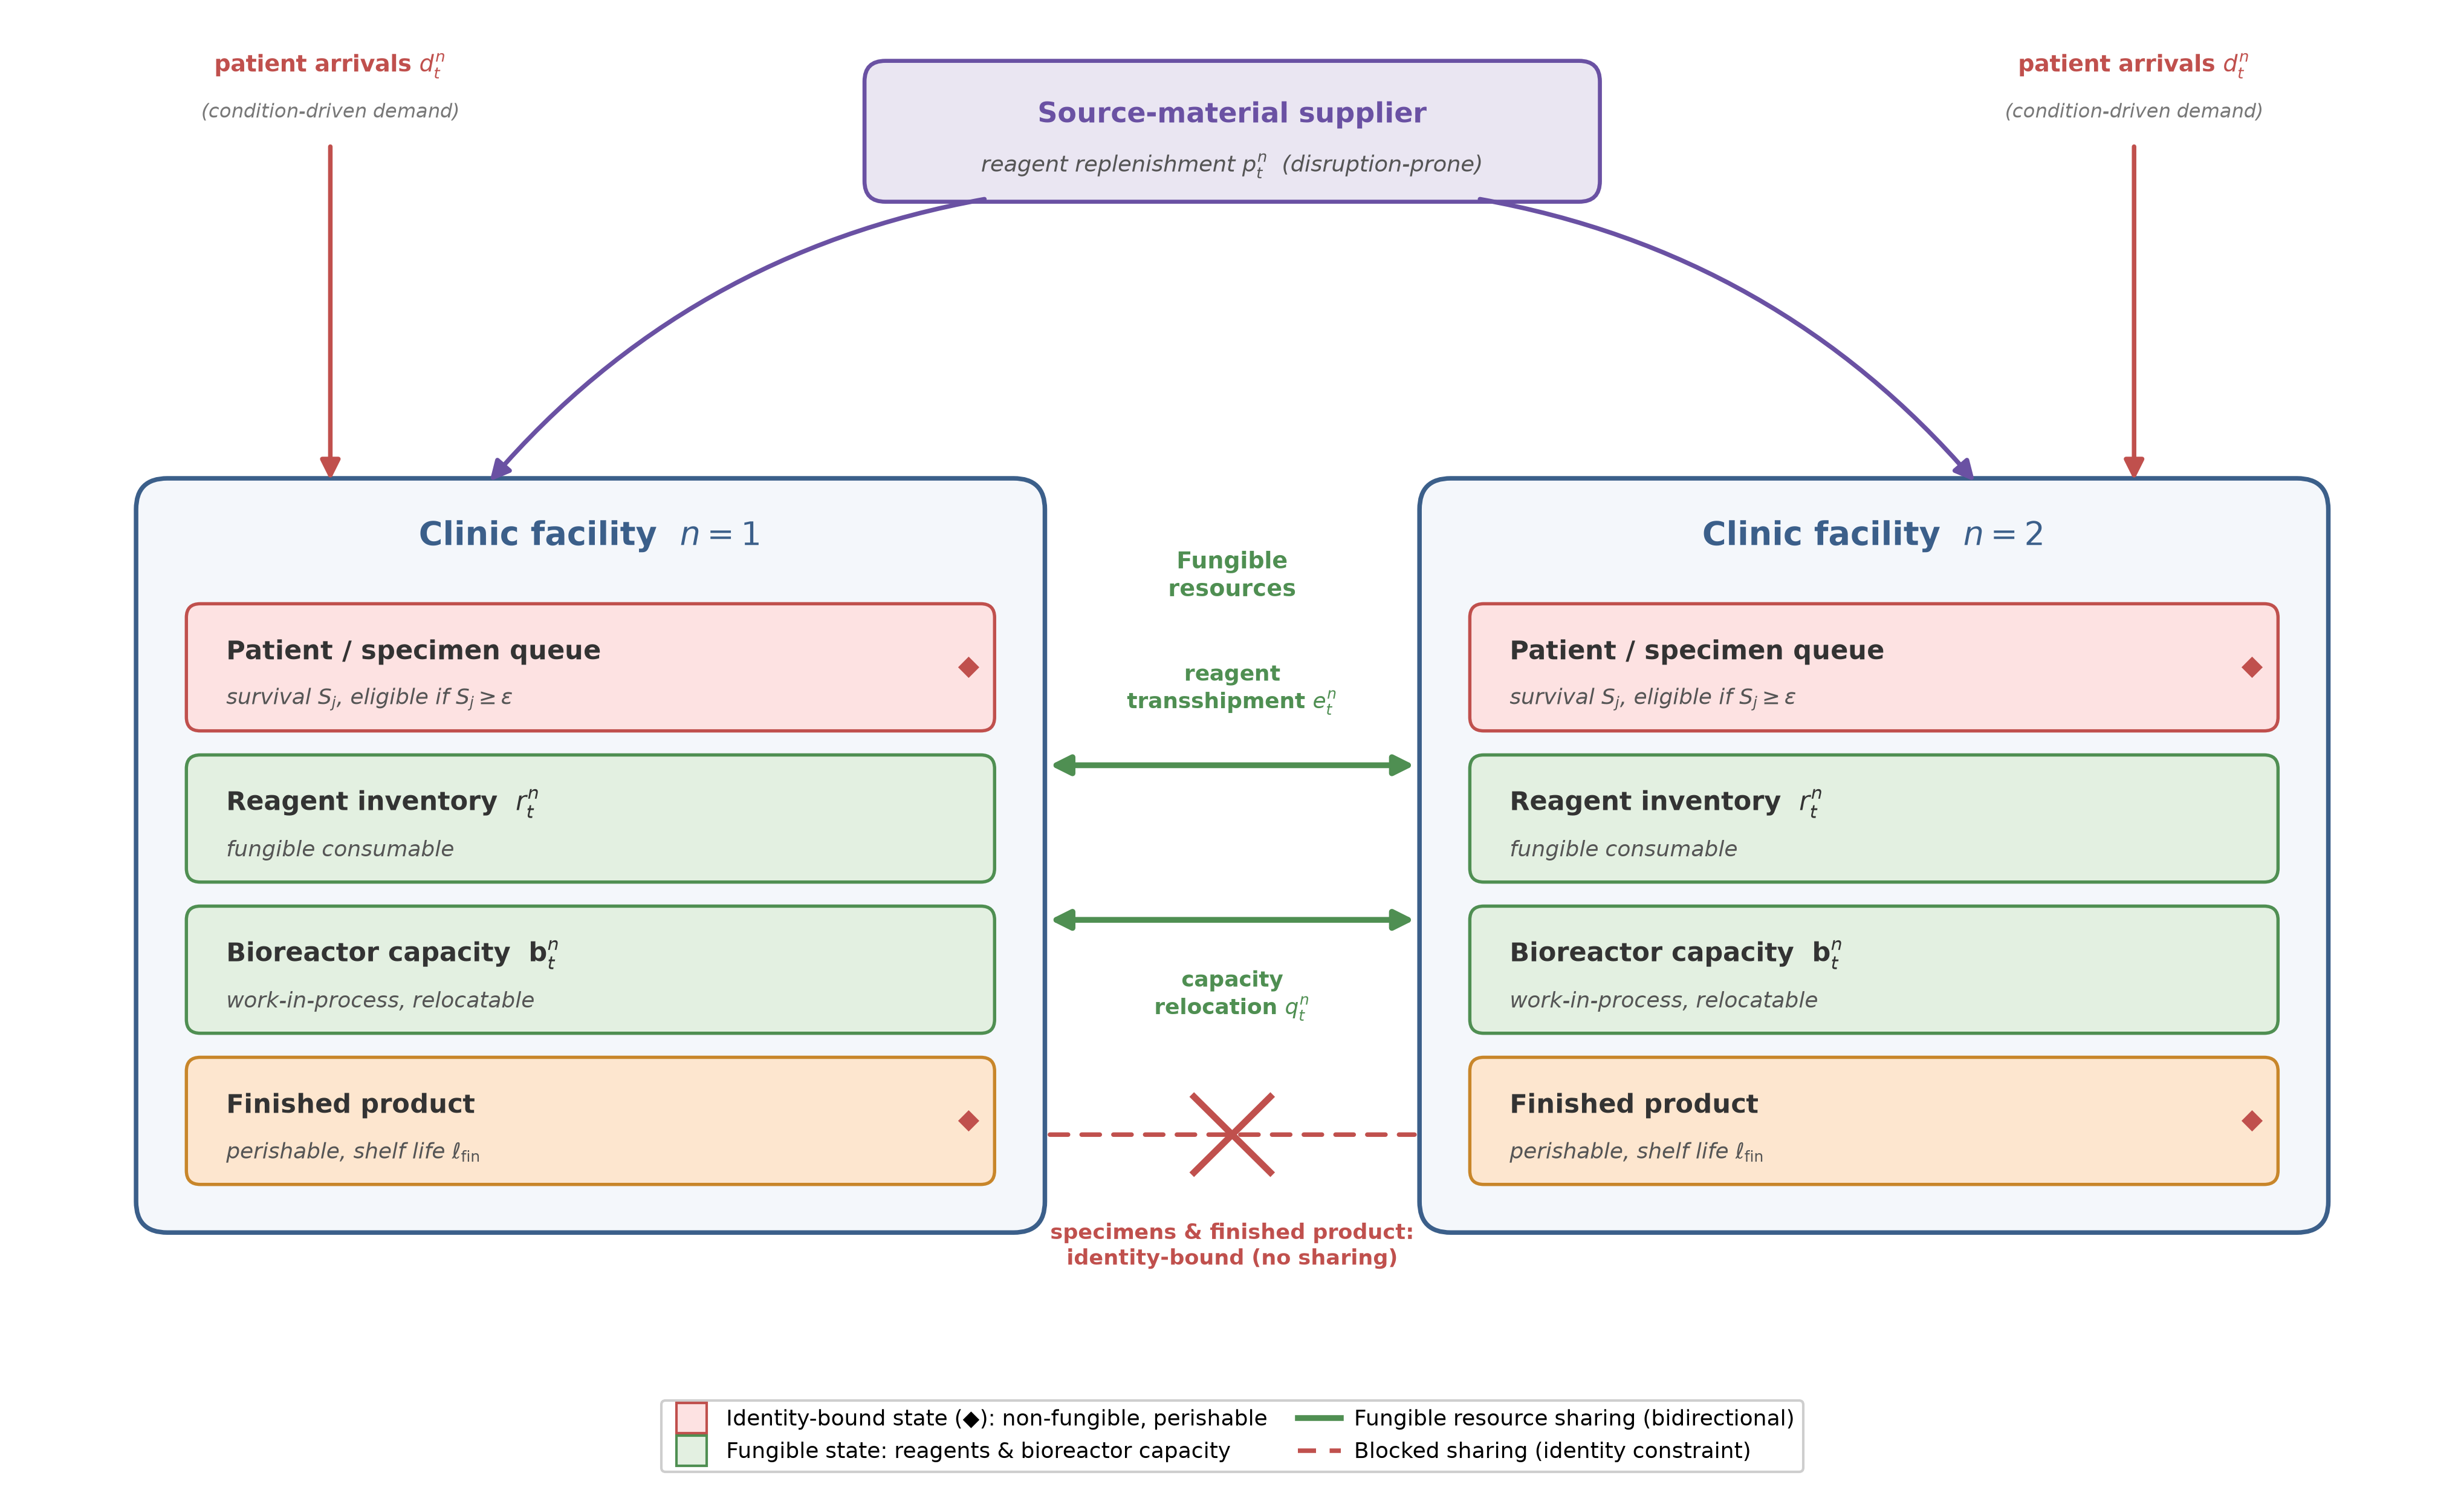
\includegraphics[width=0.95\textwidth]{figures/Figure 1.png}
    \caption{Illustration of a two-facility distributed manufacturing system for personalized regenerative medicine. Each \DIFdelbeginFL \DIFdelFL{manufacturing }\DIFdelendFL facility \DIFdelbeginFL \DIFdelFL{contains three key operational states}\DIFdelendFL \DIFaddbeginFL \DIFaddFL{holds four state components}\DIFaddendFL : \DIFdelbeginFL \DIFdelFL{the specimen demand }\DIFdelendFL \DIFaddbeginFL \DIFaddFL{a patient--specimen }\DIFaddendFL queue \DIFaddbeginFL \DIFaddFL{whose members carry a deteriorating survival index $S_j$ (eligible while $S_j \ge \epsilon$)}\DIFaddendFL , \DIFdelbeginFL \DIFdelFL{the available source material }\DIFdelendFL \DIFaddbeginFL \DIFaddFL{reagent }\DIFaddendFL inventory \DIFaddbeginFL \DIFaddFL{$r_t^n$}\DIFaddendFL , \DIFdelbeginFL \DIFdelFL{and the available production }\DIFdelendFL \DIFaddbeginFL \DIFaddFL{bioreactor }\DIFaddendFL capacity \DIFdelbeginFL \DIFdelFL{represented by bioreactors}\DIFdelendFL \DIFaddbeginFL \DIFaddFL{$\mathbf{b}_t^n$, and perishable finished product}\DIFaddendFL . \DIFdelbeginFL \DIFdelFL{Demand arrivals }\DIFdelendFL \DIFaddbeginFL \DIFaddFL{Condition-driven patient demand $d_t^n$ }\DIFaddendFL and \DIFaddbeginFL \DIFaddFL{disruption-prone }\DIFaddendFL reagent replenishment \DIFdelbeginFL \DIFdelFL{are subject to supply chain }\DIFdelendFL \DIFaddbeginFL \DIFaddFL{$p_t^n$ arrive under }\DIFaddendFL uncertainty. The \DIFdelbeginFL \DIFdelFL{bidirectional link between }\DIFdelendFL \DIFaddbeginFL \DIFaddFL{two }\emph{\DIFaddFL{fungible}} \DIFaddFL{resources---reagents and bioreactor capacity---can be rebalanced across }\DIFaddendFL facilities \DIFdelbeginFL \DIFdelFL{represents demand sharing }\DIFdelendFL \DIFaddbeginFL \DIFaddFL{through transshipment $e_t^n$ }\DIFaddendFL and capacity relocation \DIFdelbeginFL \DIFdelFL{, which allow the network to rebalance workload }\DIFdelendFL \DIFaddbeginFL \DIFaddFL{$q_t^n$ (solid green links). Patient specimens }\DIFaddendFL and \DIFdelbeginFL \DIFdelFL{resources }\DIFdelendFL \DIFaddbeginFL \DIFaddFL{finished product are }\emph{\DIFaddFL{identity-bound}}\DIFaddFL{: they cannot be pooled or reassigned }\DIFaddendFL across facilities \DIFdelbeginFL \DIFdelFL{when local demand, inventory, or capacity becomes imbalanced}\DIFdelendFL \DIFaddbeginFL \DIFaddFL{(crossed red link)}\DIFaddendFL . \DIFaddbeginFL \DIFaddFL{This fungible-only sharing under an identity constraint is the operational asymmetry that distinguishes distributed PRM manufacturing.}\DIFaddendFL }
    \label{fig:manufacturing_system}
\end{figure}

For the $N$ facilities, $T$ epochs of manufacturing time are required to produce one of the PRM products, and the planning horizon consists of $\Gamma$ epochs where $\Gamma>T$.

At epoch $t \in\{1,2, \cdots, \Gamma\}$, the production status of the $n$-th facility for $n=1, \cdots, N$ is expressed as a state vector $\mathbf{x}_{t}^{n}$, where

\begin{equation}
\mathbf{x}_{t}^{n}=\left(s_{t}^{n}, r_{t}^{n}, \mathbf{b}_{t}^{n}, P_{t}^{n}\right),
\end{equation}
Based on the state variables at epoch $t$, the facilities need to take action to adjust their production capacity for epoch $t+1$. We define the action $\mathbf{a}_{t}^{n}$ as a vector that consists of the amount of capacity sharing and reagent replenishment. The action is decided at the beginning of the production period $t$ and executed before the start of $t+1$.

\begin{equation}
\mathbf{a}_{t}^{n}=\left(w_{t}^{n}, e_{t}^{n}, q_{t}^{n}, p_{t}^{n}\right),
\end{equation}

The goal of capacity planning is to minimize total production cost by dynamically selecting the actions from Equation (2) for all facilities, denoted by $\mathbf{A}_{t}=\left(\mathbf{a}_{t}^{1}, \cdots, \mathbf{a}_{t}^{N}\right)$, for each epoch $t \in \Gamma$. We define $V\left( \mathbf{X}_{t}\right)$ as the total future cost of the selecting actions $\mathbf{A}_{t}$ when the states from all facilities, denoted by $\mathbf{X}_{t}=\left(\mathbf{x}_{t}^{1}, \cdots, \mathbf{x}_{t}^{N}\right)$, are observed at epoch $t \in \Gamma$. The objective function can be expressed as a dynamic programming problem:

\begin{equation}
\begin{array}{ll}
 V\left( \mathbf{X}_{t}\right)= 
 \min _{\mathbf{A}_{t}} & E\left[c\left(\mathbf{A}_{t} ; \mathbf{X}_{t}\right)+\gamma  V\left(\mathbf{X}_{t+1}\right)\right],
\end{array}
\end{equation}

which is useful for finding the optimal action $\mathbf{A}_{t}$ for each state $\mathbf{X}_{t}$ at each epoch $t \in \Gamma$, where $c\left(\mathbf{A}_{t} ; \mathbf{X}_{t}\right)$ is the immediate cost at time $t$, and $\gamma \in[0,1]$ is a discount factor for balancing the impact of future costs in deciding actions. The choice of $\gamma$ depends on the user's goal; if $\gamma$ is closer to 1 (to 0 ), then it means the user cares more about long (short) term cost; if $\gamma=0$, then only the cost for current epoch is considered. Equation (3) generalizes the optimality equation for the capacity planning problem in $\mathrm{Li}(2021)$ \cite{Li2023} in that cost functions \textit{$\mathbf{c}$} and $\mathbf{V}$ and the cumulative distribution function for the expectation operator can be unknown.
\DIFdelbegin \DIFdel{In the next section we will propose a DRL approach based on the DDPG algorithm for determining the solution of Equation }\DIFdelend \DIFaddbegin 

\DIFadd{Equations~(1)--}\DIFaddend (\DIFdelbegin \DIFdel{3) by learning the cost functions }\textit{\DIFdel{$\mathbf{c}$}} %DIFAUXCMD
\DIFdel{and $\mathbf{V}$ and the cumulative distribution function for the expectation operator using data-driven approaches. }\DIFdelend \DIFaddbegin \DIFadd{3) describe the base operational MDP shared with generic networked replenishment problems. The remainder of this section extends it along the three dimensions that distinguish PRM capacity planning: the deteriorating clinical condition of the patients awaiting treatment, the hard expiry of biological source material and finished product, and the autologous identity constraint that forbids pooling of patient-specific specimens. Section~\ref{sec:method} then develops a graph-aware DRL approach that learns the cost function $\mathbf{c}$, the value function $\mathbf{V}$, and the expectation operator directly from simulated experience.
}\DIFaddend 

\DIFaddbegin \subsection{\DIFadd{Patient condition and treatment eligibility}}
\label{sec:problem-patient}

\DIFadd{In generic capacity planning, a unit of unmet demand is deferred, backordered, or lost at a fixed penalty, and its value does not change while it waits. PRM demand behaves differently: each arrival is a patient whose clinical condition deteriorates over time, so a specimen that waits too long yields---if it yields anything---a product for a patient who is no longer eligible to receive it. We therefore attach an explicit condition process to every waiting patient.
}

\DIFadd{When a patient $j$ enrolls at facility $n$, we draw a latent health index $H_j \sim \mathrm{Uniform}(0,1)$ and a deterioration epoch $\tau_j \sim \theta\,\mathrm{Weibull}(\kappa)$ with shape $\kappa$ and scale $\theta$; $H_j$ captures the heterogeneous baseline robustness across patients, while $\tau_j$ marks the onset of accelerated decline. Let $\alpha_j$ be the number of epochs the patient has waited. The patient's survival index $S_j \in [0,1]$---a normalized proxy for the likelihood that the patient remains treatable---evolves as
}

\begin{equation}
\DIFadd{\label{eq:survival}
S_j(\alpha_j) = \ell(\alpha_j) + H_j\big(u(\alpha_j) - \ell(\alpha_j)\big),
}\end{equation}
\DIFadd{where $u(\alpha)=\exp\!\big(-\lambda_H\,g(\alpha)\big)$ and $\ell(\alpha)=\exp\!\big(-\lambda_F\,g(\alpha)\big)$ are the survival trajectories of an ideally healthy and a maximally frail patient, with decay rates $\lambda_H < \lambda_F$, so that $H_j$ interpolates each patient between the two bounds. The effective exposure time
}

\begin{equation}
\DIFadd{\label{eq:effective-time}
g(\alpha) =
\begin{cases}
\alpha, & \alpha \le \tau_j,\\[2pt]
\tau_j + \rho\,(\alpha - \tau_j), & \alpha > \tau_j,
\end{cases}
}\end{equation}
\DIFadd{accelerates by a factor $\rho > 1$ once the patient passes the deterioration epoch $\tau_j$, reflecting the clinically observed transition to rapid decline. A patient remains eligible for treatment only while $S_j \ge \epsilon$; once $S_j$ crosses the eligibility threshold $\epsilon$, the patient can no longer benefit from the therapy and leaves the queue as an }\emph{\DIFadd{ineligibility loss}}\DIFadd{. Because condition erodes monotonically in expectation and accelerates after $\tau_j$, waiting is not a neutral buffering decision but an irreversible loss of realizable demand---an aspect absent from classical inventory and capacity models. Parameter values are reported in Section~\ref{sec:experiments}.
}

\subsection{\DIFadd{Perishability of materials and finished product}}
\label{sec:problem-expiry}

\DIFadd{Both the biological source material and the finished product are perishable and identity-specific, so they cannot be stockpiled against future demand. A waiting specimen that is not put into production within $\ell_{\mathrm{mat}}$ epochs of enrollment expires: the patient is lost and the reserved material is wasted. Finished product that is not delivered within $\ell_{\mathrm{fin}}$ epochs of completion likewise expires and is discarded. We track, per facility $n$ and epoch $t$, the patients lost to ineligibility $\phi^{n,\mathrm{elig}}_t$ and to specimen expiry $\phi^{n,\mathrm{exp}}_t$, and the finished units lost to expiry $\psi^{n,\mathrm{fin}}_t$. It is convenient to collect the total patients lost and total material wasted at each facility,
}

\begin{equation}
\DIFadd{\label{eq:loss-aggregates}
\phi^{n}_t = \phi^{n,\mathrm{elig}}_t + \phi^{n,\mathrm{exp}}_t,
\qquad
\psi^{n}_t = \phi^{n,\mathrm{exp}}_t + \psi^{n,\mathrm{fin}}_t,
}\end{equation}
\DIFadd{where an expired specimen contributes both a lost patient and a unit of wasted material. To signal impending losses before they occur, we also count the }\emph{\DIFadd{at-risk unserved}} \DIFadd{patients whose survival has fallen within an urgency margin $\delta$ of the eligibility boundary, $\upsilon^{n}_t = \big|\{\, j \text{ waiting at } n : S_j < \epsilon + \delta \,\}\big|$.
}

\subsection{\DIFadd{Autologous identity constraint and admissible transfers}}
\label{sec:problem-identity}

\DIFadd{The autologous nature of PRM imposes a constraint with no analog in commodity supply chains: a specimen and the product manufactured from it are bound to a single patient and cannot be substituted, pooled, or delivered to anyone else. Consequently, although the network may rebalance fungible resources---reagents and bioreactor capacity---across facilities, it can never transship specimens or finished product to serve another facility's demand. In the notation of Equation~(2) this fixes the specimen-adjustment component to $w^n_t \equiv 0$ for all $n$ and $t$, so the effective per-facility decision reduces to reagent transfer $e^n_t$, capacity relocation $q^n_t$, and reagent purchase $p^n_t$, each subject to inventory and capacity feasibility. The network therefore moves fungible capacity toward where identity-bound work already sits, rather than moving the work toward idle capacity---the defining operational asymmetry of distributed PRM manufacturing.
}

\subsection{\DIFadd{Extended cost and the constrained graph MDP}}
\label{sec:problem-graph-mdp}

\DIFadd{The immediate cost augments the operational base cost $c_{\mathrm{op}}$---covering reagent purchase, holding, and shortage; bioreactor holding and shortage; and reagent and capacity transfer---with three condition- and perishability-driven terms:
}

\begin{equation}
\DIFadd{\label{eq:cost}
c(\mathbf{A}_t;\mathbf{X}_t) = c_{\mathrm{op}}(\mathbf{A}_t;\mathbf{X}_t)
+ \omega_{\mathrm{lost}}\!\sum_{n\in N}\phi^n_t
+ \omega_{\mathrm{exp}}\!\sum_{n\in N}\psi^n_t
+ \omega_{\mathrm{urg}}\!\sum_{n\in N}\upsilon^n_t,
}\end{equation}
\DIFadd{with weights ordered $\omega_{\mathrm{lost}} \gg \omega_{\mathrm{exp}} > \omega_{\mathrm{urg}}$ to encode the clinical priority: losing a patient dominates wasting material, which in turn dominates the shaping penalty for letting patients drift toward the eligibility boundary. The urgency term $\upsilon^n_t$ steers the controller to act pre-emptively---starting production or relocating capacity---before losses are actually incurred.
}

\DIFadd{To act on this cost, the controller needs visibility into the condition of each waiting queue. We therefore extend the facility state of Equation~(1) with a condition summary $\boldsymbol{\sigma}^n_t$,
}

\begin{equation}
\DIFadd{\label{eq:extended-state}
\tilde{\mathbf{x}}^n_t = \big(s^n_t, r^n_t, \mathbf{b}^n_t, P^n_t, \boldsymbol{\sigma}^n_t\big),
}\end{equation}
\DIFadd{where $\boldsymbol{\sigma}^n_t$ aggregates the survival distribution of the waiting patients---the number of patients within successive survival bands and the most-urgent survival level---so the policy can anticipate losses rather than merely react to realized demand.
}

\DIFadd{Finally, we cast the extended problem as a }\emph{\DIFadd{constrained graph MDP}}\DIFadd{. The facilities and their admissible reagent- and capacity-sharing links form a graph $\mathcal{G}=(N,\mathcal{E})$; specimen and finished-product edges carry no flow under the identity constraint, so only fungible-resource edges are active. The global state $\tilde{\mathbf{X}}_t=(\tilde{\mathbf{x}}^1_t,\ldots,\tilde{\mathbf{x}}^N_t)$ is a signal over the nodes of $\mathcal{G}$, and the action $\mathbf{A}_t$ assigns per-node purchases and per-edge transfers subject to $w^n_t\equiv 0$ and to inventory and capacity feasibility. The optimality equation~(3) carries over verbatim with the extended state $\tilde{\mathbf{X}}_t$ and cost~\eqref{eq:cost}, but the value function must now trade current operating cost against the future risk of patient losses and expiry. This constrained graph MDP---perishable, identity-bound, and patient-condition-driven---is the problem the remainder of the paper addresses, and its graph structure is precisely what the method of Section~\ref{sec:method} is designed to exploit.
}


\DIFaddend \section{Literature Review}
\label{sec:literature}

\DIFaddbegin \DIFadd{We review three bodies of work that our approach draws together: the operations of personalized regenerative medicine (PRM) and decentralized manufacturing; reinforcement learning and graph learning for networked operational decisions; and the underlying method foundations of continuous-control reinforcement learning and graph neural networks. Rather than surveying each exhaustively, we read them as an argument: each stream supplies part of what a distributed PRM capacity-planning controller needs, none supplies all of it, and together they imply a small set of design choices that we make explicit at the end of the section. Throughout, we treat the learning machinery as established and concede that graph representation and reinforcement learning have already been combined for supply-chain problems; what remains open is the PRM problem itself---perishable, identity-bound, and patient-condition-driven.
}

\DIFaddend \subsection{Personalized regenerative medicine and decentralized manufacturing}
PRM supply chains differ substantially from conventional make-to-stock manufacturing systems because products are individualized, time-sensitive, and tightly coupled with patient-specific clinical pathways. In autologous cell therapy, patient material must be collected, transported, manufactured, quality-tested, and returned for administration, and manufacturing can begin only when a specimen, consumables, and production capacity are jointly available. These characteristics make fulfillment time, service reliability, and resource utilization central operational measures. Wang et al.~\cite{Wang2023SimulationBased} used simulation to compare centralized and point-of-care autologous cell therapy supply chain strategies and evaluated cost, fulfillment time, service level, and resource utilization. Li and White~\cite{Li2023} further studied decentralized autologous cell therapy manufacturing networks and showed that transshipment and relocatable capacity can reduce the cost of resilience under supplier disruption.

These studies establish that PRM network design and inter-facility coordination are first-order engineering decisions rather than implementation details. Related work on cell therapy manufacturing process control also highlights the potential of reinforcement learning in uncertain, nonlinear, and partially observed manufacturing environments~\cite{Zheng2022HybridMBRL}. Together, this literature motivates a data-driven decision-support framework that can represent both the temporal dynamics of patient-specific manufacturing and the spatial dependencies created by distributed facilities.

\subsection{Reinforcement learning for supply chain and manufacturing decisions}
Reinforcement learning has been widely studied for sequential supply chain and manufacturing decisions. Early work applied RL to inventory replenishment in multi-echelon supply chains and perishable inventory systems~\cite{GIANNOCCARO2002153,KARA2018150}. More recent studies have used deep reinforcement learning to handle high-dimensional state spaces, stochastic demand, and simulation-based decision environments. For example, Oroojlooyjadid et al.~\DIFdelbegin \DIFdel{\mbox{%DIFAUXCMD
\cite{article1} }\hskip0pt%DIFAUXCMD
}\DIFdelend \DIFaddbegin \DIFadd{\mbox{%DIFAUXCMD
\cite{Oroojlooyjadid2022BeerGame} }\hskip0pt%DIFAUXCMD
}\DIFaddend developed a deep Q-network approach for the beer game, demonstrating that DRL can learn replenishment policies in decentralized, partially observed supply chain settings.
\DIFdelbegin \DIFdel{Wang et al.~\mbox{%DIFAUXCMD
\cite{article2} }\hskip0pt%DIFAUXCMD
combined reinforcement learning with multi-agent simulation for dynamic inventory replenishment in an aerospace manufacturing supply chain.
}\DIFdelend 

Recent supply chain RL studies have moved toward more realistic constraints and engineering settings. Bermudez et al.~\cite{Bermudez2023DCPO} proposed distributional constrained reinforcement learning for multi-period supply chain optimization with production and inventory constraints. Eisenach et al.~\cite{Eisenach2024NeuralCoordination} studied shared-resource capacity control in inventory management using a neural coordination mechanism and a reinforcement learning buying policy. Stranieri et al.~\cite{Stranieri2025PharmaDRL} benchmarked classical and deep reinforcement learning inventory policies for pharmaceutical supply chains with perishability and non-stationary demand. These studies support the use of simulation-trained RL policies for uncertain operational control, but most focus on replenishment or inventory management rather than the joint capacity, \DIFdelbegin \DIFdel{inventory, specimen transshipment, and demand-sharing decisions that }\DIFdelend \DIFaddbegin \DIFadd{reagent, and replenishment decisions---under a perishable, identity-bound demand process---that }\DIFaddend arise in distributed PRM manufacturing.

\subsection{Deep reinforcement learning for regenerative medicine capacity planning}
The closest antecedent to this work is Tseng et al.~\cite{Tseng2023DeepRL}, who developed a deep reinforcement learning approach for dynamic capacity planning in decentralized regenerative medicine supply chains. Their study demonstrated that simulation-trained policies can adapt to demand and supply uncertainty without requiring exact prior knowledge of the underlying stochastic processes. This is directly aligned with the objective of using data-driven policy learning for PRM capacity planning.

The present study builds on this line of work by adding an explicit graph representation layer to encode inter-facility relationships. In decentralized PRM networks, facilities are linked through \DIFdelbegin \DIFdel{possible demand sharing, reagent transshipment , and capacity relocation}\DIFdelend \DIFaddbegin \DIFadd{reagent transshipment and bioreactor capacity relocation, whereas patient specimens and finished product remain identity-bound}\DIFaddend . Therefore, a facility's decision depends not only on its own local state but also on the states and \DIFaddbegin \DIFadd{fungible-}\DIFaddend resource conditions of connected facilities. A flat vectorized state representation can include all facility variables, but it does not explicitly exploit the graph structure that governs how information and resources propagate across the network. This motivates \DIFdelbegin \DIFdel{the integration of }\DIFdelend \DIFaddbegin \DIFadd{integrating }\DIFaddend graph convolutional representation learning with \DIFdelbegin \DIFdel{deep deterministic policy gradient }\DIFdelend \DIFaddbegin \DIFadd{continuous-control actor--critic reinforcement }\DIFaddend learning.

\subsection{Multi-agent reinforcement learning and graph learning for networked supply chains}
Recent multi-agent reinforcement learning studies are relevant because distributed manufacturing networks naturally involve decentralized information and coordinated actions. Mousa et al.~\cite{Mousa2023DecInvMARL} formulated decentralized inventory control as a multi-agent problem and studied centralized-training/decentralized-execution policies under local information constraints. Leluc et al.~\cite{Leluc2023MARLIM} similarly demonstrated the promise of cooperative multi-agent reinforcement learning for inventory management under stochastic demand and lead times. These studies show that decentralization is not only an application feature but also an algorithmic design dimension.

In parallel, graph neural networks have emerged as a natural representation tool for supply chains and other networked operational systems. Chang et al.~\cite{Chang2025AAAI} learned production functions on supply-chain graphs using temporal graph neural networks and an inventory module, showing the value of explicit relational structure for supply-chain inference and forecasting. Ahn et al.~\cite{Ahn2024GSP} used attention-based graph neural networks for probabilistic supply and inventory prediction in enterprise supply-chain networks, while Ahn et al.~\cite{Ahn2024GPP} combined graph neural networks, offline reinforcement learning, and policy simulation for dynamic supply planning. Kotecha and del Rio Chanona~\cite{Kotecha2024GNNMARL} are particularly relevant because they combine graph neural network state representations with multi-agent reinforcement learning for supply chain inventory control. These studies collectively suggest that graph-based learning is useful for networked supply chain systems; however, most existing work remains focused on prediction, inventory-only control, or general supply-chain planning rather than continuous-action control of PRM-specific capacity, reagent, and specimen flows.

\DIFaddbegin \subsection{\DIFadd{Method foundations: continuous-control reinforcement learning and graph neural networks}}
\DIFadd{The decisions in our problem---capacity relocation, reagent replenishment, and consumable transfer---are real-valued, which points to continuous-control actor--critic methods. Deterministic policy gradients and DDPG~\mbox{%DIFAUXCMD
\cite{Lillicrap2016DDPG} }\hskip0pt%DIFAUXCMD
extended actor--critic learning to continuous action spaces, but are known to suffer from value overestimation and training instability. TD3~\mbox{%DIFAUXCMD
\cite{Fujimoto2018TD3} }\hskip0pt%DIFAUXCMD
mitigates overestimation through clipped double-$Q$ learning, delayed policy updates, and target smoothing; SAC~\mbox{%DIFAUXCMD
\cite{Haarnoja2018SAC} }\hskip0pt%DIFAUXCMD
adds entropy regularization for more robust exploration and stability; and PPO~\mbox{%DIFAUXCMD
\cite{Schulman2017PPO} }\hskip0pt%DIFAUXCMD
is a widely used on-policy alternative built on a clipped surrogate objective. The practical implication is that DDPG, though historically the default for continuous supply-chain control, is no longer an uncontested choice: a defensible study should compare backbones rather than commit to one, and should expect the more stable off-policy methods to reduce the run-to-run variance that plagues DDPG.
}

\DIFadd{Graph neural networks encode relational structure through neighborhood aggregation. The graph convolutional network~\mbox{%DIFAUXCMD
\cite{Kipf2017GCN} }\hskip0pt%DIFAUXCMD
and its successors---GraphSAGE~\mbox{%DIFAUXCMD
\cite{Hamilton2017GraphSAGE} }\hskip0pt%DIFAUXCMD
for inductive neighborhood sampling and graph attention networks~\mbox{%DIFAUXCMD
\cite{Velickovic2018GAT} }\hskip0pt%DIFAUXCMD
for learned edge weighting---provide a permutation-equivariant inductive bias that a flat multilayer perceptron lacks. Coupling such encoders with reinforcement learning has become a recognized paradigm for networked decision problems~\mbox{%DIFAUXCMD
\cite{Liu2024GNNMARLSurvey}}\hskip0pt%DIFAUXCMD
. For a clinic network whose facilities interact through capacity relocation and consumable transshipment, this relational bias is a modeling choice of substance rather than convenience: it allows a single policy to reason over the topology along which shortages, slack, and disruptions propagate.
}

\DIFaddend \subsection{Evaluation considerations for deep reinforcement learning}
Evaluation rigor is especially important for DRL-based engineering applications. Henderson et al.~\cite{Henderson2018DRLMatters} showed that deep reinforcement learning results can be sensitive to random seeds, hyperparameters, and implementation details. Agarwal et al.~\cite{Agarwal2021RLiable} further argued that few-run comparisons can be statistically unreliable and recommended more robust aggregate metrics and interval estimates. These findings imply that a DRL-based supply chain study should report implementation details, training budgets, out-of-sample test procedures, and variability across replications or random seeds when possible. In the present study, we therefore emphasize common simulation settings across all benchmark policies, detailed implementation parameters for the \DIFdelbegin \DIFdel{GCN-DDPG agent}\DIFdelend \DIFaddbegin \DIFadd{graph-aware actor--critic agents}\DIFaddend , and Monte Carlo evaluation under multiple disruption and demand forecast scenarios\DIFaddbegin \DIFadd{, with interquartile-mean performance and confidence intervals reported across random seeds}\DIFaddend .

\begin{table}[htbp]
\centering
\small
\caption{Positioning of this study relative to closely related literature.}
\label{tab:lit_positioning}
\setlength{\tabcolsep}{4pt}
\renewcommand{\arraystretch}{1.12}
\begin{tabularx}{\textwidth}{p{0.24\textwidth} p{0.27\textwidth} X}
\toprule
Literature stream & Representative studies & Main limitation relative to this work \\
\midrule
PRM and autologous cell therapy operations & Simulation and decentralized capacity planning studies~\cite{Wang2023SimulationBased,Li2023,Tseng2023DeepRL} & Establish the need for adaptive PRM capacity planning, but do not \DIFdelbeginFL \DIFdelFL{explicitly }\DIFdelendFL learn graph-structured inter-facility representations for continuous coordinated control\DIFaddbeginFL \DIFaddFL{, nor model product perishability, patient-condition-driven demand, or the autologous identity constraint}\DIFaddendFL . \\
RL for supply chain and manufacturing & DRL inventory, replenishment, and constrained supply chain control~\DIFdelbeginFL \DIFdelFL{\mbox{%DIFAUXCMD
\cite{article1,article2,Bermudez2023DCPO,Stranieri2025PharmaDRL,Eisenach2024NeuralCoordination} }\hskip0pt%DIFAUXCMD
}\DIFdelendFL \DIFaddbeginFL \DIFaddFL{\mbox{%DIFAUXCMD
\cite{Oroojlooyjadid2022BeerGame,Bermudez2023DCPO,Stranieri2025PharmaDRL,Eisenach2024NeuralCoordination} }\hskip0pt%DIFAUXCMD
}\DIFaddendFL & Demonstrate simulation-trained policies, but mainly focus on inventory or replenishment rather than \DIFaddbeginFL \DIFaddFL{the }\DIFaddendFL coupled capacity, reagent, and specimen-flow decisions \DIFaddbeginFL \DIFaddFL{of patient-specific manufacturing}\DIFaddendFL . \\
MARL for decentralized supply chains & Decentralized inventory and cooperative inventory management~\cite{Mousa2023DecInvMARL,Leluc2023MARLIM} & Address decentralized information and coordination, but are not tailored to PRM manufacturing or patient-specific make-to-order constraints. \\
GNNs for supply chain networks & Supply-chain graph forecasting, supply prediction, and graph-aware inventory control~\cite{Chang2025AAAI,Ahn2024GSP,Ahn2024GPP,Kotecha2024GNNMARL} & Show the value of graph structure, but are mostly predictive, inventory-focused, or not designed for PRM capacity and transshipment control. \\
\bottomrule
\end{tabularx}
\end{table}

\subsection{Research gap \DIFaddbegin \DIFadd{and design implications}\DIFaddend }
\DIFdelbegin \DIFdel{The literature indicates three important trends. First, PRM manufacturing requires adaptive capacity planning because patient-specific demand, consumable availability, and production capacity jointly determine treatment fulfillment. Second, reinforcement learning provides a data-driven approach for sequential operational decisions under uncertainty. Third, graph neural networks provide a natural representation for supply chains and distributed manufacturing networks with relational dependencies. Nevertheless, limited work has integrated graph convolutional representation learning with }\DIFdelend \DIFaddbegin \DIFadd{Read together, these literatures imply four design choices for a distributed PRM capacity-planning controller. }\emph{\DIFadd{(i)}} \DIFadd{Because the decisions are sequential and real-valued, the controller should use continuous-control }\DIFaddend actor--critic reinforcement learning \DIFdelbegin \DIFdel{for distributed PRM manufacturing networks}\DIFdelend \DIFaddbegin \DIFadd{rather than value-based or discretized methods. }\emph{\DIFadd{(ii)}} \DIFadd{Because a facility's value depends on its network position and resources propagate along inter-facility links, the state should be encoded with a graph representation rather than a flat vector. }\emph{\DIFadd{(iii)}} \DIFadd{Because DDPG is prone to instability and has been superseded on stability grounds, the study should compare backbones---TD3, SAC, and PPO alongside DDPG---and treat DDPG as an ablation rather than the proposed method. }\emph{\DIFadd{(iv)}} \DIFadd{Because deep reinforcement learning results are sensitive to seeds and implementation details, evaluation should go beyond mean cost, reporting multi-seed interquartile means and confidence intervals and, given the clinical stakes, patient-service outcomes such as eligibility and waiting}\DIFaddend .

\DIFdelbegin \DIFdel{Published PRM operations studies establish }\DIFdelend \DIFaddbegin \DIFadd{These implications are necessary but not sufficient, because none of the reviewed streams addresses the problem that defines our setting. PRM operations research establishes }\DIFaddend the need for \DIFdelbegin \DIFdel{distributed capacity planning under uncertainty, but they are predominantly simulation, OR, ADP, or flat-state DRL based. Recent supply chain RL studies show that simulation-trained policies can handle stochastic inventory and capacity-control problems, but they usually flatten network state or focus on replenishment rather than jointly modeling capacity relocation, consumables, and specimen transshipment. Recent GNN studies show that supply chains are natively graph structured, yet much of this work remains predictive or inventory-focused. This study addresses the gap by developing a GCN-DDPG framework that learns a }\DIFdelend \DIFaddbegin \DIFadd{adaptive, networked capacity planning but does not learn relational policies; supply-chain graph-and-reinforcement-learning research supplies the relational-control machinery but represents demand as fungible, abstract requests and targets forecasting, inventory-only control, or generic enterprise planning; and cell-therapy reinforcement learning operates at the level of a single bioprocess rather than a network of clinics. Consequently, no prior work models the three properties that make PRM capacity planning distinct---a perishable product with a hard viability deadline, an identity-bound product that cannot be pooled or substituted across patients, and demand driven by patient deterioration while waiting---within a single }\DIFaddend graph-aware \DIFdelbegin \DIFdel{continuous-action policy for distributed PRM manufacturing under supplier disruption and demand forecast error. The framework is positioned as an intelligent engineering decision-support system rather than only a domain-specific application of DDPG}\DIFdelend \DIFaddbegin \DIFadd{continuous-control formulation. Closing that gap, and providing a simulation testbed in which it can be studied, is the contribution of this paper}\DIFaddend .

\section{Graph-Aware Deep Reinforcement Learning Framework}
\label{sec:method}
\DIFdelbegin \textbf{\DIFdel{Integrating DDPG with GCN for Distributed Manufacturing (DDPG-GCN):}}
%DIFAUXCMD
\DIFdelend \DIFaddbegin \subsection*{\DIFadd{Overview: a shared graph encoder with interchangeable actor--critic backbones}}
\DIFaddend 

\DIFdelbegin \subsection*{\DIFdel{Introduction to the Method}}
%DIFAUXCMD
%DIFDELCMD < 

%DIFDELCMD < %%%
\DIFdel{distributed }\DIFdelend \DIFaddbegin \DIFadd{Distributed }\DIFaddend manufacturing networks for \DIFdelbegin \DIFdel{Personalized Regenerative Medicine }\DIFdelend \DIFaddbegin \DIFadd{personalized regenerative medicine }\DIFaddend (PRM) \DIFdelbegin \DIFdel{involve }\DIFdelend \DIFaddbegin \DIFadd{comprise }\DIFaddend complex, interconnected facilities whose operating states are best represented as graphs rather than flat vectors. Classical reinforcement learning \DIFdelbegin \DIFdel{(RL) models, which treat }\DIFdelend \DIFaddbegin \DIFadd{that treats }\DIFaddend each facility as independent \DIFdelbegin \DIFdel{,
struggle to }\DIFdelend \DIFaddbegin \DIFadd{cannot }\DIFaddend capture these spatial dependencies. \DIFdelbegin \DIFdel{To address this, we integrate the Deep Deterministic
Policy Gradient (DDPG) algorithm with a Graph Convolutional Network }\DIFdelend \DIFaddbegin \DIFadd{We therefore adopt a two-part design shared by every method we study: a graph convolutional network }\DIFaddend (GCN) \DIFdelbegin \DIFdel{, enabling the agent to learn joint capacityand transshipment decisions while accounting for network structure}\DIFdelend \DIFaddbegin \DIFadd{encoder that maps the networked state to permutation-equivariant, neighborhood-aware node embeddings, composed with a continuous-control actor--critic backbone that maps those embeddings to feasibility-projected capacity, reagent, and replenishment actions. Writing the controller as }\emph{\DIFadd{encoder $\circ$ backbone}} \DIFadd{lets us hold the relational representation fixed while swapping the reinforcement-learning backbone, so that any performance difference between backbones is attributable to the learning algorithm rather than to the state representation}\DIFaddend .

\subsection*{Rationale\DIFdelbegin \DIFdel{for the DDPG-GCN Integration}\DIFdelend \DIFaddbegin \DIFadd{: why a family of backbones rather than a single algorithm}\DIFaddend }

\DIFdelbegin \DIFdel{The DDPGalgorithm is well suited }\DIFdelend \DIFaddbegin \DIFadd{Consistent with the design implications drawn in Section~\ref{sec:literature}, we do not commit to a single backbone. We evaluate a family of continuous-control actor--critic algorithms behind the shared GCN encoder (Table~\ref{tab:backbone_family}). Deep deterministic policy gradient (DDPG) is the classical off-policy actor--critic }\DIFaddend for continuous control\DIFdelbegin \DIFdel{problems, providing a model-free, off-policy }\DIFdelend \DIFaddbegin \DIFadd{; because it is prone to value overestimation and run-to-run instability, we treat the GCN--DDPG pairing as a baseline and ablation rather than as the proposed method. TD3, SAC, and PPO are the stability-oriented backbones we expect to reduce the variance that plagues DDPG: TD3 through clipped double-$Q$ learning, delayed policy updates, and target smoothing; SAC through entropy-regularized stochastic policies; and PPO through an on-policy clipped surrogate objective. All four share the encoder, the feasibility-projection layer, and the environment, so the comparison is controlled. A GCN encodes relational structure but has no temporal memory of its own; the }\DIFaddend actor--critic \DIFdelbegin \DIFdel{mechanism for policy learning. However, DDPG alone assumes vectorized
inputs and cannot directly leverage the relational information among facilities. Conversely, GCNs
excel at extracting structural embeddings from graph-structured data but lack temporal learning
capabilities. Their integration allows the model to }\DIFdelend \DIFaddbegin \DIFadd{backbone supplies the sequential decision dynamics, and the two together }\DIFaddend encode spatial correlations \DIFdelbegin \DIFdel{through GCN layers
and temporal decision dynamics through DDPGupdates. 
}\DIFdelend \DIFaddbegin \DIFadd{and temporal trade-offs jointly.
}\DIFaddend 

\DIFaddbegin \begin{table}[htbp]
\centering
\small
\caption{\DIFaddFL{Continuous-control actor--critic backbones evaluated behind the shared GCN encoder.}}
\label{tab:backbone_family}
\setlength{\tabcolsep}{4pt}
\renewcommand{\arraystretch}{1.15}
\begin{tabularx}{\textwidth}{p{0.10\textwidth} p{0.13\textwidth} p{0.11\textwidth} X}
\toprule
\DIFaddFL{Backbone }& \DIFaddFL{Policy class }& \DIFaddFL{Sampling }& \DIFaddFL{Key mechanism and role in this study }\\
\midrule
\DIFaddFL{DDPG~\mbox{%DIFAUXCMD
\cite{Lillicrap2016DDPG} }\hskip0pt%DIFAUXCMD
}& \DIFaddFL{Deterministic }& \DIFaddFL{Off-policy }& \DIFaddFL{Baseline actor--critic for continuous control; value overestimation and training instability motivate treating GCN--DDPG as an ablation rather than the proposed method. }\\
\DIFaddFL{TD3~\mbox{%DIFAUXCMD
\cite{Fujimoto2018TD3} }\hskip0pt%DIFAUXCMD
}& \DIFaddFL{Deterministic }& \DIFaddFL{Off-policy }& \DIFaddFL{Clipped double-$Q$ learning, delayed policy updates, and target smoothing to curb overestimation and stabilize training. }\\
\DIFaddFL{SAC~\mbox{%DIFAUXCMD
\cite{Haarnoja2018SAC} }\hskip0pt%DIFAUXCMD
}& \DIFaddFL{Stochastic }& \DIFaddFL{Off-policy }& \DIFaddFL{Entropy-regularized objective for more robust exploration and training stability. }\\
\DIFaddFL{PPO~\mbox{%DIFAUXCMD
\cite{Schulman2017PPO} }\hskip0pt%DIFAUXCMD
}& \DIFaddFL{Stochastic }& \DIFaddFL{On-policy }& \DIFaddFL{Clipped surrogate objective; an on-policy alternative to the off-policy backbones. }\\
\bottomrule
\end{tabularx}
\end{table}

\DIFadd{For concreteness we present the framework in full for the DDPG instantiation---the GCN encoder, the actor--critic updates, and the feasibility projection---and then note where each stability-oriented backbone modifies the critic target, the policy parameterization, or the update schedule; the GCN encoder and the feasibility-projection layer are identical across backbones.
}

\DIFaddend Figure~\ref{fig:graph_structure} shows the graph abstraction used \DIFdelbegin \DIFdel{in the proposed GCN-DDPG }\DIFdelend \DIFaddbegin \DIFadd{by the proposed graph-aware }\DIFaddend framework. Each healthcare clinic is represented as a node with facility-specific state features, including waiting specimens \DIFaddbegin \DIFadd{and their condition summary}\DIFaddend , reagent inventory, available bioreactor capacity, and other local operational conditions. The edges encode different forms of inter-facility dependency. Information-flow edges \DIFdelbegin \DIFdel{allow the model to share demand and operational }\DIFdelend \DIFaddbegin \DIFadd{let the model propagate operational and patient-condition }\DIFaddend signals among neighboring clinics; resource-sharing edges represent feasible reagent \DIFdelbegin \DIFdel{or specimen }\DIFdelend transshipment relationships; and capacity-sharing edges connect each clinic to the central capacity hub. \DIFaddbegin \DIFadd{Consistent with the autologous identity constraint, only fungible reagents and bioreactor capacity flow along edges---specimens and finished product remain node-local. }\DIFaddend By applying graph convolution over this structure, the model learns a network-aware representation in which each facility's decision is informed not only by its own state but also by the states of connected facilities. This graph embedding is then passed to the \DIFdelbegin \DIFdel{DDPG }\DIFdelend actor--critic \DIFdelbegin \DIFdel{networks }\DIFdelend \DIFaddbegin \DIFadd{backbone }\DIFaddend to support coordinated capacity\DIFdelbegin \DIFdel{planning and transshipment }\DIFdelend \DIFaddbegin \DIFadd{, reagent, and replenishment }\DIFaddend decisions.

\begin{figure}[htbp]
    \centering
    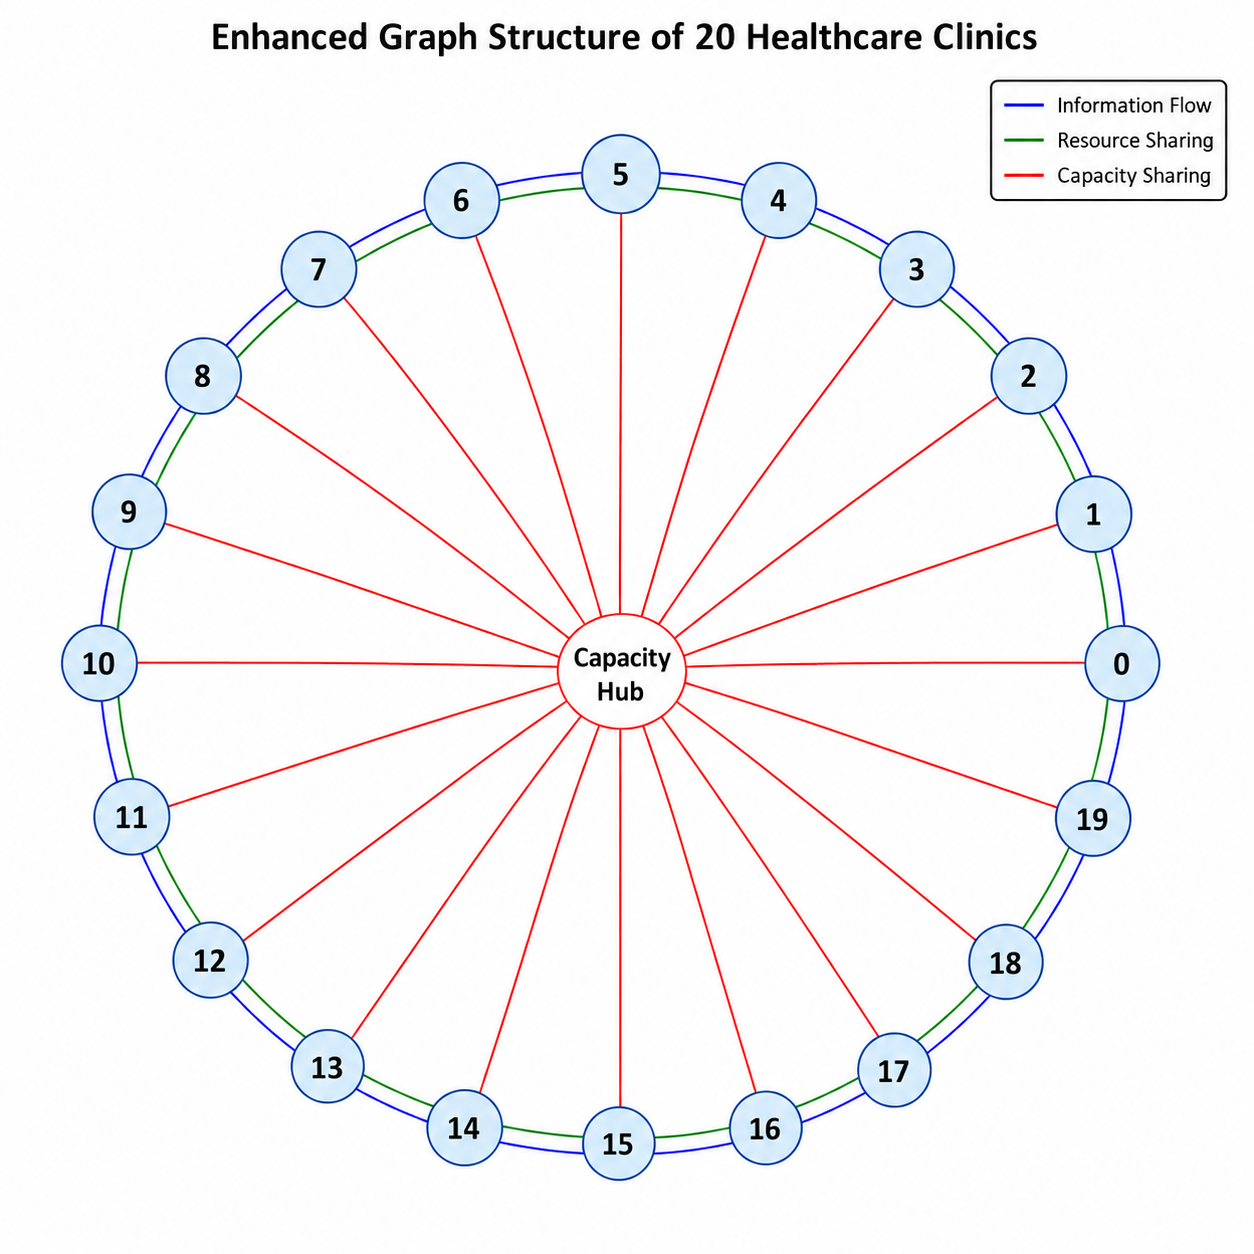
\includegraphics[width=0.78\textwidth]{figures/Figure 2.png}
    \caption{Graph representation of a distributed personalized regenerative medicine manufacturing network with 20 healthcare clinics. Each outer node represents a clinic or manufacturing facility, and the central node represents the shared capacity pool. Blue edges indicate information flow among neighboring clinics, green edges indicate resource sharing relationships, and red radial edges indicate capacity sharing between each clinic and the central capacity hub. This graph structure is used by the graph convolutional network to encode both local facility states and neighboring network information for downstream reinforcement learning decisions.}
    \label{fig:graph_structure}
\end{figure}

Formally, let $G_t=(V,E_t)$ represent the manufacturing network at epoch $t$, where each node
$v_i\in V$ denotes a facility with state features $x_i^t$ and edge weights $e_{ij}^t$ indicate
logistic or transshipment costs. The GCN encodes local and neighborhood information using a
layer-wise propagation rule:
\begin{equation}
h_i^{(l+1)} = \sigma \Big(W^{(l)} \sum_{j \in \mathcal{N}(i)} \frac{1}{c_{ij}} h_j^{(l)} \Big),
\end{equation}
where $h_i^{(0)} = x_i^t$, $W^{(l)}$ are trainable weights, $\sigma(\cdot)$ is a ReLU activation,
and $c_{ij}$ is a degree-based normalization factor. The resulting embedding
$H_t = \{h_i^{(L)}\}_{i=1}^{N}$ captures the current global state of the network.
\subsection*{Overview of the \DIFdelbegin \DIFdel{DDPG-GCN Workflow}\DIFdelend \DIFaddbegin \DIFadd{graph-aware actor--critic workflow (DDPG instantiation)}\DIFaddend }

The method initiates with a dual initialization: the \DIFdelbegin \DIFdel{DDPG's }\DIFdelend actor and critic networks \DIFaddbegin \DIFadd{of the backbone }\DIFaddend and the GCN for graph state processing. Given an observed state \( X_t \), represented as raw graph data reflecting the current status of the manufacturing network, the GCN is used as a preprocessing unit. It transforms this raw graph into a condensed representation \( X'_t \), which retains the critical structural information of the original graph.

Following this transformation, the DDPG algorithm gets involved. Using the graph-processed state \( X'_t \), the actor-network selects an action, which is based on the actor--critic architecture. This action could range from decisions regarding resource allocation to inventory replenishments. Once executed within the manufacturing environment, the system provides a feedback loop in the form of a reward, essentially evaluating the decision's efficacy.

The DDPG then uses this feedback, in tandem with the replay buffer, to refine both the actor and critic networks, ensuring better decision-making in subsequent iterations. The GCN, on its part, continuously updates its understanding of the graph structure as the manufacturing network evolves, ensuring it remains adaptive and accurate in its representations.


\subsection*{Initialization}
\begin{itemize}
\item Critic network \( Q(X_t, A_t|\theta_Q) \) initialized with weights \( \theta_Q \).
\item Actor network \( \mu(X_t|\theta_\mu) \) initialized with weights \( \theta_\mu \).
\item GCN initialized with weights \( \omega \) for processing graph states.
\end{itemize}

\subsection*{DDPG Component}
The DDPG agent operates on the GCN-encoded state $H_t$ to generate an action vector 
$A_t = \{\mathbf{a}_i^t\}_{i=1}^{N}$, where $\mathbf{a}_i^t$ specifies the capacity adjustment,
inventory replenishment, and transshipment quantities for facility $i$. 
The actor network $\mu(H_t|\theta_\mu)$ outputs continuous actions, while the critic network
$Q(H_t,A_t|\theta_Q)$ estimates the expected cumulative cost. The optimization follows the standard
DDPG updates:
\begin{align}
y_i &= c_i(A_i;H_i) + \gamma Q'(H_{i+1},\mu'(H_{i+1}|\theta_{\mu'})|\theta_{Q'}),\\
L_Q &= \frac{1}{N}\sum_i (y_i - Q(H_i,A_i|\theta_Q))^2,\\
\nabla_{\theta_\mu} J &= \frac{1}{N}\sum_i \nabla_a Q(H_i,a|\theta_Q)|_{a=\mu(H_i)} 
\nabla_{\theta_\mu} \mu(H_i|\theta_\mu).
\end{align}

\subsection*{Reward \DIFdelbegin \DIFdel{Function}\DIFdelend \DIFaddbegin \DIFadd{function}\DIFaddend }
The \DIFdelbegin \DIFdel{reward (negative cost) encourages policies that balance cost minimization and service-level
stability}\DIFdelend \DIFaddbegin \DIFadd{agents optimize the negative of the immediate cost defined in Section~\ref{sec:problem-graph-mdp}}\DIFaddend . For each epoch $t$, the \DIFdelbegin \DIFdel{immediate reward is
defined as
}\begin{displaymath}
\DIFdel{r_t = -\Big( C_t^{\text{reagent}} + C_t^{\text{bio}} + C_t^{\text{trans}} \Big),
}\end{displaymath}%DIFAUXCMD
\DIFdelend \DIFaddbegin \DIFadd{reward is
}\begin{equation}
\DIFadd{r_t = -\,c(\mathbf{A}_t;\tilde{\mathbf{X}}_t),
}\end{equation}\DIFaddend 
where \DIFdelbegin \DIFdel{each term corresponds to the reagent, bioreactor, and transshipment cost components
introduced in Eq. ~(14). This formulation allows }\DIFdelend \DIFaddbegin \DIFadd{$c(\cdot)$ is the extended cost of Equation~\eqref{eq:cost}, comprising the operational base cost $c_{\mathrm{op}}$ (reagent purchase, holding, and shortage; bioreactor holding and shortage; and reagent and capacity transfer) together with the patient-loss, material-and-product-expiry, and urgency terms. Optimizing this reward therefore requires }\DIFaddend the agent to \DIFdelbegin \DIFdel{learn trade-offs between resource utilization and timely delivery}\DIFdelend \DIFaddbegin \DIFadd{trade current operating cost against the future risk of patient losses and expiry, rather than resource utilization alone}\DIFaddend .


\begin{algorithm}[p]
\footnotesize
\caption{\DIFdelbegin \DIFdel{DDPG--GCN }\DIFdelend \DIFaddbegin \DIFadd{Graph-aware actor--critic }\DIFaddend for \DIFdelbegin \DIFdel{Distributed }\DIFdelend \DIFaddbegin \DIFadd{distributed }\DIFaddend PRM \DIFdelbegin \DIFdel{Capacity Planning}\DIFdelend \DIFaddbegin \DIFadd{capacity planning (DDPG instantiation; TD3/SAC/PPO swap the critic target, policy parameterization, or update schedule).}\DIFaddend }
\label{alg:ddpg_gcn}
\begin{algorithmic}[1]
\Require Discount factor $\gamma$, soft-update rate $\tau$, actor and critic learning rates $\alpha_\mu,\alpha_Q$, exploration scale $\sigma$, minibatch size $N$.
\State Initialize GCN encoder $g_\omega$, actor $\mu(\cdot\mid\theta_\mu)$, critic $Q(\cdot,\cdot\mid\theta_Q)$, target networks $\mu'$ and $Q'$, and replay buffer $\mathcal{R}$.
\For{each environment step $t$}
    \State Observe raw graph state $X_t$ and compute graph embedding $Z_t=g_\omega(X_t)$.
    \State Select exploratory action $A_t=\mu(Z_t\mid\theta_\mu)+\epsilon_t$, where $\epsilon_t\sim\mathcal{N}(0,\sigma^2 I)$.
    \State Project or clip $A_t$ to the feasible set and execute the resulting action $\hat{A}_t$.
    \State Observe cost/reward $r_t$, next state $X_{t+1}$, and store $(X_t,\hat{A}_t,r_t,X_{t+1})$ in $\mathcal{R}$.
    \If{an update is scheduled}
        \State Sample minibatch $(X_i,A_i,r_i,X_{i+1})_{i=1}^{N}$ from $\mathcal{R}$ and compute $Z_i=g_\omega(X_i)$, $Z_{i+1}=g_\omega(X_{i+1})$.
        \State Compute targets $y_i=r_i+\gamma Q'(Z_{i+1},\mu'(Z_{i+1}\mid\theta_{\mu'})\mid\theta_{Q'})$.
        \State Update critic by minimizing $L_Q=N^{-1}\sum_i(y_i-Q(Z_i,A_i\mid\theta_Q))^2$.
        \State Update actor using the deterministic policy gradient $\nabla_{\theta_\mu}J$.
        \State Backpropagate through the GCN encoder and softly update target networks.
    \EndIf
\EndFor
\State \Return trained actor $\mu(g_\omega(X)\mid\theta_\mu)$.
\end{algorithmic}
\end{algorithm}

\paragraph{Action decoding and feasibility projection.}
Because the actor network outputs continuous actions, an additional deterministic decoding and feasibility-projection step is used before actions are executed in the simulation environment. Let $A_t^{\mathrm{raw}}=\mu(Z_t|\theta_\mu)$ denote the raw continuous action generated by the actor network from the graph embedding $Z_t$. The raw action is first scaled to the admissible range of each decision variable and then clipped to its variable-specific lower and upper bounds. \DIFdelbegin \DIFdel{Integer-valued operational quantities, including specimen reassignment, reagent }\DIFdelend \DIFaddbegin \DIFadd{Under the autologous identity constraint the specimen-adjustment component is fixed to zero, so the decoded decision comprises only the fungible quantities---reagent }\DIFaddend transshipment, bioreactor relocation, and \DIFdelbegin \DIFdel{replenishment quantities, }\DIFdelend \DIFaddbegin \DIFadd{replenishment---which }\DIFaddend are then rounded to the nearest feasible integer values.

The decoded action is subsequently passed through a repair operator that enforces the operational constraints of the manufacturing network. First, nonnegativity constraints are imposed so that the resulting action cannot remove more \DIFdelbegin \DIFdel{specimens, reagents , }\DIFdelend \DIFaddbegin \DIFadd{reagents }\DIFaddend or idle bioreactors from a facility than are available at that epoch. Second, replenishment quantities are capped by the maximum purchasable reagent quantity $P_t^n$ and by supplier availability. Third, network conservation constraints are enforced for \DIFdelbegin \DIFdel{internal }\DIFdelend \DIFaddbegin \DIFadd{the fungible }\DIFaddend sharing decisions: the total \DIFdelbegin \DIFdel{number of specimens, reagents , }\DIFdelend \DIFaddbegin \DIFadd{quantities of reagents }\DIFaddend and relocatable bioreactors sent out from facilities must equal the total amount received by connected facilities, except for external reagent purchases\DIFaddbegin \DIFadd{; specimens and finished product are identity-bound and are never transferred}\DIFaddend . Finally, transshipment and relocation actions are restricted to feasible graph edges; if no edge connects two facilities, the corresponding flow is set to zero.

Equivalently, the executed action can be interpreted as the feasible action $\hat{A}_t$ obtained by projecting the decoded actor output onto the feasible action set $\mathcal{F}(X_t)$:
\DIFdelbegin %DIFDELCMD < [
%DIFDELCMD < %%%
\DIFdel{$\hat{A}_t = \Pi_{\mathcal{F}(X_t)}(A_t^{\mathrm{raw}}),$
}%DIFDELCMD < ]
%DIFDELCMD < %%%
\DIFdelend \DIFaddbegin \begin{equation}
\DIFadd{\hat{A}_t = \Pi_{\mathcal{F}(X_t)}\!\left(A_t^{\mathrm{raw}}\right),
}\end{equation}
\DIFaddend where $\mathcal{F}(X_t)$ is determined by current facility states, inventory availability, capacity availability, supplier limits, \DIFaddbegin \DIFadd{the autologous identity constraint, }\DIFaddend and graph connectivity. This projection step improves engineering credibility by ensuring that all actions executed in the simulation correspond to implementable capacity, replenishment, and transshipment decisions.


\DIFdelbegin %DIFDELCMD < \vspace{0.3em}
%DIFDELCMD < \noindent%%%
\textbf{\DIFdel{GCN Encoder:}} %DIFAUXCMD
\DIFdel{Each facility node $i$ aggregates features from its neighbors $\mathcal{N}(i)$ using layer-wise message passing:
}\[
\DIFdel{h_i^{(l+1)} = \sigma\!\left(W^{(l)} \sum_{j \in \mathcal{N}(i)} h_j^{(l)}\right),
}\]%DIFAUXCMD
\DIFdel{where $W^{(l)}$ are trainable weights and $\sigma(\cdot)$ is an activation function. 
This produces graph-embedded representations used by the actor–critic networks for coordinated decision-making. }%DIFDELCMD < 

%DIFDELCMD < %%%
\subsection*{\DIFdel{Anticipated Outcomes and Benefits}}
%DIFAUXCMD
%DIFDELCMD < 

%DIFDELCMD < %%%
\DIFdel{The DDPG-GCN model offers several tangible benefits:
}%DIFDELCMD < 

%DIFDELCMD < \begin{itemize}
\begin{itemize}%DIFAUXCMD
%DIFDELCMD <     \item %%%
\item%DIFAUXCMD
\textbf{\DIFdel{Enhanced Prediction and Analysis}}%DIFAUXCMD
\DIFdel{: By leveraging the relationships between clinics, our GCN framework can generate predictions with greater accuracy and nuanced analysis, surpassing the capabilities of models that consider clinics in isolation.
    }%DIFDELCMD < \item %%%
\item%DIFAUXCMD
\textbf{\DIFdel{Pattern Identification}}%DIFAUXCMD
\DIFdel{: The GCN is adept at detecting trends and patterns that may extend across multiple clinics, thereby uncovering insights that isolated analyses could overlook.
    }%DIFDELCMD < \item %%%
\item%DIFAUXCMD
\textbf{\DIFdel{Efficient Graph Processing}}%DIFAUXCMD
\DIFdel{: By harnessing the power of GCNs, the model can effectively handle states that are naturally represented as graphs, ensuring no critical information is lost in translation.
    }%DIFDELCMD < \item %%%
\item%DIFAUXCMD
\textbf{\DIFdel{Optimized Decision-Making}}%DIFAUXCMD
\DIFdel{: The DDPG component ensures that the actions selected are both contextually relevant (thanks to the GCN-processed states) and optimal in terms of the overall system objectives.
    }%DIFDELCMD < \item %%%
\item%DIFAUXCMD
\textbf{\DIFdel{Adaptive Learning}}%DIFAUXCMD
\DIFdel{: As the manufacturing network evolves, both the DDPG and GCN components continuously refine their parameters, ensuring the model remains adaptive and responsive to real-world changes. }
\end{itemize}%DIFAUXCMD
%DIFDELCMD < \end{itemize}
%DIFDELCMD < 

%DIFDELCMD < %%%
\DIFdel{In essence, the integration offers a solution that is greater than the sum of its parts, paving the way for more efficient, resilient, and optimized distributed manufacturing systems}\DIFdelend \DIFaddbegin \DIFadd{Each stability-oriented backbone reuses this encoder and projection layer unchanged and alters only the reinforcement-learning update. TD3 replaces the single critic with clipped double-$Q$ targets, delays actor updates, and adds target-policy smoothing; SAC replaces the deterministic actor with an entropy-regularized stochastic policy and a soft value target; and PPO replaces off-policy replay with on-policy rollouts optimized under a clipped surrogate objective. In all cases the actor and critic operate on the GCN embedding $Z_t$ rather than on the flat state, and the executed action is the feasibility-projected $\hat{A}_t$}\DIFaddend .

\DIFdelbegin \DIFdel{This proposed DDPG-GCN model offers a robust approach for distributed manufacturing. By melding the strengths of GCN and DDPG, it provides a nuanced understanding of intricate manufacturing networks, ensuring efficient and optimized decision-making.
The dynamic nature and intricate dependencies found in distributed manufacturing necessitate advanced solutions capable of understanding and optimizing such networks. The integration of DDPG and GCN, as presented in this paper, provides a promising avenue for addressing the challenges inherent in distributed manufacturing systems. With the capability to process graph-based states effectively, the DDPG-GCN model offers substantial improvements in service level, efficiency, and resilience against disruptions}\DIFdelend \DIFaddbegin \subsection*{\DIFadd{Summary}}

\DIFadd{The framework is thus a single graph-aware controller with a swappable actor--critic core: a GCN encoder supplies a permutation-equivariant, network-aware state representation; a continuous-control backbone learns coordinated capacity, reagent, and replenishment policies from simulated experience; and a deterministic feasibility-projection layer guarantees that every executed action respects inventory, capacity, supplier, identity, and connectivity constraints. Holding the encoder and projection fixed while varying the backbone lets the experiments in Section~\ref{sec:experiments} separate the value of the graph representation from that of the reinforcement-learning algorithm, and compare DDPG against the more stable TD3, SAC, and PPO on equal footing}\DIFaddend .
\section{Computational Experiments}
\label{sec:experiments}
\label{sec:casestudies}

This section presents two case studies designed to evaluate the efficacy of the proposed DDPG-GCN framework in a distributed PRM manufacturing system. The case studies aim to illustrate the framework's adaptability to varying demand forecast accuracies and its capacity for making informed decisions within a complex network of interconnected clinics. The experiments are designed to compare the learned graph-aware policy with heuristic and look-ahead policies under the same simulation environment, which helps isolate the value of adaptive policy learning under disruption and forecast error.
\subsection{Objective}
The objective of this study is to compare the performance of the proposed GCN-DDPG (Graph Convolutional Network - Deep Deterministic Policy Gradient) framework with traditional heuristic methods in the context of distributed manufacturing.

\subsection{Methodology}

\subsubsection{Benchmarking Setup}
To evaluate both the value of reinforcement learning and the value of graph-based representation learning, we compare the proposed GCN-DDPG framework with two groups of baselines. The first group consists of traditional heuristic and look-ahead policies implemented in the same simulation environment. These baselines provide domain-relevant comparisons with existing capacity planning approaches. The second group consists of learning-based ablations designed to isolate the contribution of the GCN encoder.

The heuristic baselines are:
\begin{itemize}
\item \textbf{MYO (Myopic):} This heuristic minimizes single-period cost without considering future demand.
\item \textbf{MDL-1 (One-period Mean Demand Lookahead):} MDL-1 extends the planning horizon to one lookahead period using deterministic state transitions based on mean demand.
\item \textbf{MDL-2 (Two-period Mean Demand Lookahead):} MDL-2 extends the planning horizon to two lookahead periods using deterministic state transitions based on mean demand.
\item \textbf{ISO (Isolated Regional Facilities):} ISO assumes no resource sharing between facilities and focuses only on local replenishment decisions.
\end{itemize}

The learning-based baseline is:
\begin{itemize}
\item \textbf{MLP-DDPG / flat-state DDPG:} This baseline uses the same DDPG actor--critic structure and the same action space as the proposed method, but removes the GCN encoder. Instead, all facility-level states are concatenated into a flat vector and passed directly into multilayer perceptron actor and critic networks. This baseline is designed to answer whether performance improvements come from reinforcement learning alone or from explicitly encoding graph-structured inter-facility dependencies.
\end{itemize}

In addition, graph ablation experiments are planned to evaluate the role of different edge types. Specifically, we consider removing capacity-sharing edges and removing resource-sharing edges to assess whether these relational structures contribute to policy performance under disruption and demand uncertainty.

\subsubsection{Performance Metrics}

We evaluate each method using both cost-based and engineering-relevant performance metrics. The primary metric is the average total cost over the planning horizon, including reagent replenishment cost, bioreactor holding and shortage penalties, and transshipment or relocation costs. To strengthen the application relevance of the experiments, we also track the following secondary metrics:
\begin{itemize}
    \item \textbf{Service level:} the fraction of patient demand that can be started or fulfilled within the planning horizon.
    \item \textbf{Average waiting time / fulfillment delay:} the average number of epochs that patient specimens wait before manufacturing begins.
    \item \textbf{Reagent shortage frequency:} the frequency with which manufacturing is delayed because insufficient reagents are available.
    \item \textbf{Bioreactor utilization:} the fraction of available bioreactor capacity used for production across facilities.
    \item \textbf{Transshipment and relocation activity:} the total number of specimen, reagent, and bioreactor movements across the network.
    \item \textbf{Inference time:} the computational time required for a trained policy or heuristic to generate one epoch-level decision.
\end{itemize}

These metrics are included because the objective of PRM capacity planning is not only to reduce operational cost, but also to support timely patient-specific manufacturing, effective resource utilization, and reliable system performance under demand and supply uncertainty.

\subsubsection{Heuristic Implementations}
We provide brief descriptions of the heuristic methods implemented:
\begin{itemize}
    \item \textbf{MYO (Myopic):} MYO focuses on minimizing costs within the current period without considering future consequences.
    \item \textbf{MDL-1 and MDL-2:} These methods extend the planning horizon to one and two lookahead periods, respectively, using deterministic state transitions based on mean demand.
    \item \textbf{ISO (Isolated Regional Facilities):} ISO assumes no sharing of resources between manufacturing facilities and primarily concentrates on reagent replenishment.
\end{itemize}

\subsubsection{GCN-DDPG Implementation}
The model is implemented in \texttt{Python 3.10} using \texttt{PyTorch}. 
The GCN encoder contains two convolutional layers with 64 and 32 hidden units, respectively, 
followed by ReLU activations. 
The DDPG actor and critic each consist of three fully connected layers with dimensions (256, 128, 64).
All parameters are initialized with Xavier initialization. 
Training uses the Adam optimizer with learning rates of $1\times10^{-4}$ for the actor and 
$1\times10^{-3}$ for the critic. 
The replay buffer size is $10^6$, minibatch size is 256, discount factor $\gamma=0.99$, 
and target update rate $\tau=0.005$. 
Exploration noise follows a decaying Ornstein–Uhlenbeck process with initial $\sigma=0.2$. 
Each model is trained for $1.0\times10^6$ steps and evaluated on 500 Monte Carlo test runs to 
ensure robustness. All experiments are conducted on an NVIDIA RTX 4090 GPU. 

This implementation ensures reproducibility and stability while maintaining scalability across
larger network configurations.
\subsection{distributed manufacturing simulation}
% Algorithm for state normalization with changed variables
\begin{algorithm}
\caption{State normalization}
\begin{algorithmic}[1]
\Require State variables: $s_t^n$, $r_t^n$, $b_t^n$, and $p_t^n$ \\
         Maximal values of the state variables for all facilities: $M_s$, $M_r$, $M_b$, and $M_p$
\Ensure Normalized state variables: $\hat{s}_t^n$, $\hat{r}_t^n$, $\hat{b}_t^n$, $\hat{p}_t^n$

\For{$n = 1$ to $N$}
    \State $\hat{s}_t^n = s_t^n / M_s$
    \State $\hat{r}_t^n = r_t^n / M_r$
    \State $\hat{b}_t^n = b_t^n / M_b$
    \State $\hat{p}_t^n = p_t^n / M_p$
\EndFor
\end{algorithmic}
\end{algorithm}

To evaluate the proposed method, we now construct a simulation environment of a decentralized manufacturing system consisting of $N=20$ manufacturing facilities and its dedicated reagent supplier. Each PRM product requires $T=3$ epochs of manufacturing time, and the considered finite problem horizon contains $\Gamma=52$ decision epochs. For every epoch $t$, there will be $d_{t}^{n}$ new demand for facility $n$. The demand arrival process for facility $n$ follows a Poisson distribution $\text{Poisson}\left(\lambda_{n}\right)$. The supplier disruption follows independent Bernoulli processes $\text{Ber}\left(\zeta_{n}\right)$, i.e., the facility $n$ has a probability $\zeta_{n}$ to have supplier disruption and could not purchase any reagent for the epoch. This simulation can be further adjusted to reflect any real situation, e.g., supply disruption and demand uncertainty, that may be encountered. Such flexibility in using the simulation system will be demonstrated in Section 5.4 when we compare GCN-DDPG with other methods.

The epoch is assumed to occur weekly, and the transshipment of specimens, bioreactors, and reagents at epoch $t$ arrive before epoch $t+1$. After the demand and source materials have arrived, the next observing state can be expressed by $\mathbf{x}_{t+1}^{n}=\left(s_{t+1}^{n}, r_{t+1}^{n}, \mathbf{b}^{n}, P_{t+1}\right)$ for facility $n=1, \ldots, N$, according to definition Equation (1). The state variables are updated by the following rules:

\begin{align*}
s_{t+1}^{n}&=s_{t}^{n}-m_{t}^{n}+d_{t}^{n}+w_{t}^{n} \\
r_{t+1}^{n}&=r_{t}^{n}-m_{t}^{n}+e_{t}^{n}+p_{t}^{n} \\
b_{t+1}^{n, \tau}&= \begin{cases}
b_{t}^{n, 0}-m_{t}^{n}+b_{t}^{n, 1}+q_{t}^{n} & \text{if } \tau=0 \\
b_{t}^{n, \tau+1} & \text{if } 1 \leq \tau \leq T-2 \\
m_{t}^{n} & \text{if } \tau=T-1
\end{cases}
\end{align*}

where $m_{t}^{n}=\min \left(s_{t}^{n}, b_{t}^{n, 0}, r_{t}^{n}\right)$ is the number of products that begin manufacturing at epoch $t$, $d_{t}^{n}$ is the demand arriving at facility $n$ in epoch $t$, and $P_{t+1}$ follows an exogenous Markov chain from $P_{t}$. The single-period cost in period $t$ of all facility $n$ can be written as:

\begin{align*}
\mathbf{C}\left(\mathbf{A}_{t} ; \mathbf{x}_{t}\right)&=\sum_{j=t}^{\Gamma} \sum_{n=1}^{N} \mathbf{C}^{n}\left(\mathbf{w}_{t}^{n}, \mathbf{e}_{t}^{n}, \mathbf{q}_{t}^{n}, \mathbf{p}_{t}^{n} ; \mathbf{s}_{t}^{n}\right) \\
\mathbf{C}^{n}\left(\mathbf{w}_{t}^{n}, \mathbf{e}_{t}^{n}, \mathbf{q}_{t}^{n}, \mathbf{p}_{t}^{n} \mid \mathbf{s}_{t}^{n}\right)&=C_{\text{Reg}, t}^{n}+C_{\text{Bio}, t}^{n}+C_{\text{Tran}, t}^{n}
\end{align*}

where the meanings of $C_{\text{Reg}, t}^{n}$, $C_{\text{Bio}, t}^{n}$, and $C_{\text{Tran}, t}^{n}$ are summarized below.

\begin{itemize}
  \item $C_{\text{Reg}, t}^{n} = c_{R} p_{t}^{n} + h_{R}\left(r_{t+1}^{n}-s_{t+1}^{n}\right)^{+} + p_{R}\left(s_{t+1}^{n}-r_{t+1}^{n}\right)^{+}$ is the cost related to reagent at epoch $t$, including the reagent replenishment cost $c_{R} p_{t}^{n}$, the reagent overstock holding cost $h_{R}\left(r_{t+1}^{n}-s_{t+1}^{n}\right)^{+}$, and the reagent understock penalty $p_{R}\left(s_{t+1}^{n}-r_{t+1}^{n}\right)^{+}$;
  \item $C_{\text{Bio}, t}^{n} = h_{B}\left(b_{t+1}^{n, 0}-s_{t+1}^{n}\right)^{+} + p_{B}\left(s_{t+1}^{n}-b_{t+1}^{n, 0}\right)^{+}$ is the cost related to bioreactor at epoch $t$, including the bioreactor overstock holding cost $h_{B}\left(b_{t+1}^{n, 0}-s_{t+1}^{n}\right)^{+}$, and the bioreactor understock penalty $p_{B}\left(s_{t+1}^{n}-b_{t+1}^{n, 0}\right)^{+}$;
  \item $C_{\text{Tran}, t}^{n} = K_{R}\left|e_{t}^{n}\right| + K_{B}\left|q_{t}^{n}\right| + K_{S}\left|w_{t}^{n}\right|$ is the total transshipping cost at epoch $t$, including the cost of transshipping $e_{t}^{n}$ units of reagent from/to facility $n$, the cost of relocating $q_{t}^{n}$ bioreactors from/to facility $n$, and the cost of transshipping $w_{t}^{n}$ specimens from facility $i$to facility $n$.
\end{itemize}


\subsection{Case Study 1: Interconnected Clinic Network Analysis}
\label{subsec:casestudy1}

 In this case study, we assume the demand forecast for heuristics is accurate and compare the cost performance of GCN-DDPG with the heuristics under three levels of supply disruption rate. This case study aims to demonstrate that
GCN-DDPG can learn effective policies under different uncertainty scenarios. Figure 3
illustrates the average total cost of GCN-DDPG and the heuristics under 0.05, 0.3 and
0.6 supplier disruption rates. The result of MYO is omitted in the figure due to its
poor performance. The result shows that GCN-DDPG can achieve comparable cost performance with the heuristics when the supplier disruption rate is low, e.g., 0.05 and
0.3. When the supplier disruption rate is high, e.g., 0.6, GCN-DDPG outperforms all
the heuristics. The cost differences between GCN-DDPG and heuristics are calculated by
$(Cost_{Heuristic}- Cost_{GCN-DDPG})/Cost_{Heuristic}\times 100$ and listed in Table 1.

\subsubsection{Results} The results indicate that the GCN-DDPG framework can leverage network-level information to improve resource allocation and respond to demand changes more effectively.
 \begin{figure}[ht]
    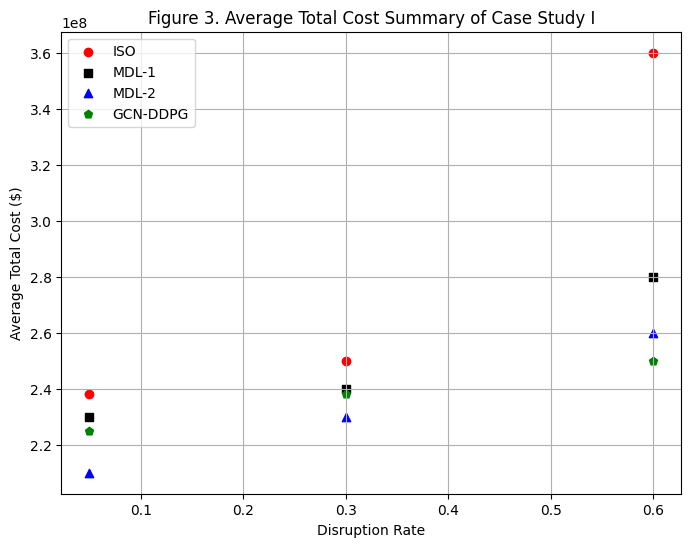
\includegraphics[width=0.85\textwidth]{Result_1.png}
            \caption{Average total cost summary of case study 1.}
 \end{figure}
 \begin{table}[h]
\centering
\caption{Cost performance comparison of case study I (\% increase)}

\begin{tabular}{lccc}
\hline
Method & \multicolumn{3}{c}{Disruption Rate} \\
\cline{2-4}
 & 0.05 & 0.3 & 0.6 \\
\hline
ISO & 5.46\% & 4.80\% & 30.56\% \\
MDL-1 & 2.17\% & 0.83\% & 10.71\% \\
MDL-2 & -7.14\% & -3.48\% & 3.85\% \\
GCN-DDPG & 0.00\% & 0.00\% & 0.00\% \\
\hline
\end{tabular}
\label{tab:cost_comparison}
\end{table}
\subsubsection{Analysis:}
The results show that GCN-DDPG performs competitively with the heuristic baselines under low and moderate disruption rates and provides clearer cost advantages under high disruption. In particular, when the supplier disruption rate is $0.6$, GCN-DDPG reduces average total cost by 30.56\% relative to ISO, 10.71\% relative to MDL-1, and 3.85\% relative to MDL-2, as reported in Table~\ref{tab:cost_comparison}. Under lower disruption rates, the cost differences are smaller, indicating that the benefit of graph-aware adaptive control becomes more visible when the network is exposed to stronger supply-side uncertainty. These results suggest that GCN-DDPG can use network-level information to support resource allocation under disruption, rather than demonstrating uniformly dominant performance across all settings. This consistent performance of GCN-DDPG underscores its potential as a scalable solution for healthcare networks, ensuring operational reliability and financial prudence even in the face of escalating disruptions.
\subsection{Case Study 2: Adaptability to Non-Stationary Demand}
\label{subsec:casestudy2}
In this case study, we assume the demand forecast is less accurate for heuristic methods. Instead, we use a range of demand levels in the simulation model for training our GCN-DDPG approach, as opposed to the actual demand distribution. This case study aims to demonstrate that GCN-DDPG can learn a single policy that can adapt to different uncertainty scenarios, mimicking a real-world application.

In the computer experiment, we let the heuristics generate capacity plans using a demand distribution \( \text{Poisson}(d) \) and \( d = \frac{250}{52} \). We then set the actual demand distribution as \( \text{Poisson}(d') \), where \( d' = d + \epsilon \cdot d \) and \( \epsilon \in \{-0.2, 0, 0.2, 0.3, 0.4, 0.5\} \), to generate data for testing heuristic methods. This approach tests the adaptability of our GCN-DDPG model to demand forecast errors that are \(-20\%, 0\%, 20\%, 30\%, 40\%, 50\% \). In addition to the constant error, we also consider scenarios of non-stationary errors where the demand forecast error changes over time as listed in Table \ref{table:nonstationary_error_design}.
 The average total cost of GCN-DDPG and the heuristics under different levels of demand forecasting accuracy are summarized
in Figure 4.
\subsubsection{Results} The results indicate that the GCN-DDPG framework can leverage network-level information to improve resource allocation and respond to demand changes more effectively.
 \begin{figure}[ht]
    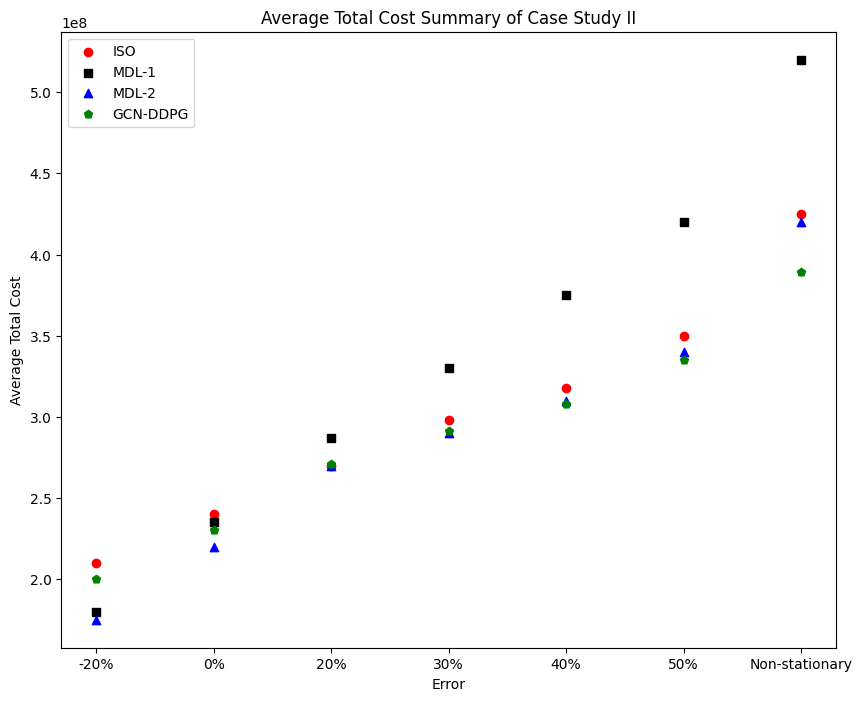
\includegraphics[width=0.85\textwidth]{Result-2.png}
            \caption{Average total cost summary of case study 2.}
 \end{figure}


We train the GCN-DDPG model to make effective capacity planning decisions under different uncertainty scenarios. The capacity planning model for the GCN-DDPG approach utilizes a uniform parameter \( \text{Uniform}(d,2d) \) for each time step, ensuring adaptability to the varying demand patterns.
\begin{table}[ht]
\centering
\caption{Summary of non-stationary demand forecast error design for Case Study II across 20 clinics.}
\label{table:nonstationary_error_design}
\begin{tabular}{c c}
\hline
Epoch & Error Rate Across Clinics \\
\hline
1-13 & Varies from 30\% to 60\%, alternating between clinics \\
14-26 & Varies from 10\% to 80\%, alternating between clinics \\
27-39 & Varies from 50\% to 100\%, alternating between clinics \\
40-52 & Varies from 40\% to 60\%, alternating between clinics \\
\hline
\end{tabular}
\end{table}


\subsubsection{Analysis}
The results indicate that GCN-DDPG achieves lower average total cost than the heuristic baselines in the higher forecast-error scenarios, including the 40\%, 50\%, and non-stationary demand-error settings. In lower-error scenarios, its performance is closer to the look-ahead heuristics, suggesting that the advantage of adaptive learning becomes more visible when the actual demand process deviates substantially from the forecast used by deterministic baselines.
\section{Discussion and Conclusions}
\label{sec:conclusion}
The two case studies conducted provide a comprehensive comparison between the cost performance of the proposed GCN-DDPG framework and four ADP-based methods under conditions where demand distributions are known a priori. The findings affirm that GCN-DDPG can generate effective actions and policies, demonstrating performance on par with ADP-based methods across various uncertainty scenarios. In the second case study, we explored scenarios where the actual demand distribution is unknown, training a single GCN-DDPG policy to address this uncertainty. The results endorse the framework's capability to learn and control capacity planning effectively under diverse demand uncertainty scenarios, thereby highlighting its applicability to real-world problems where system uncertainties are unknown.

While the capacity planning problem we explored is inspired by PRM manufacturing, the flexibility of the GCN-DDPG approach suggests its potential applicability across a wide range of manufacturing applications to enhance supply chain resilience, even without a predefined system structure.


The GCN-DDPG framework, leveraging the power of simulation and the learning capabilities of Deep Reinforcement Learning, is particularly well-suited for modeling complex systems and learning optimal control policies. This approach offers significant benefits for PRM supply chains, including the ability to make immediate decisions using a neural network-based trained policy, avoiding the need for time-consuming optimization processes typical of analytical methods. Furthermore, a well-trained GCN-DDPG policy can be adapted to different system settings, such as varying levels of demand uncertainty, without the necessity for retraining.

However, challenges remain in the deployment of GCN-DDPG within PRM supply chains. Achieving acceptable performance with DRL policies may require meticulous hyperparameter tuning or extended training times. The simulation environment must accurately reflect the supply chain's state to allow for efficient retraining and maintenance of policies. Significant changes in the system may necessitate policy retraining to ensure the quality of decisions. Practitioners must develop a robust workflow for training, maintaining, and validating GCN-DDPG policies to mitigate the risk of suboptimal decision-making.

\textbf{Future Work}
This study motivates several potential research extensions. First, the simulation
model can be improved by adding variables such as patient health condition, raw material quality, product quality, process failure rate, machine breakdown process, and operator availability. Furthermore, other PRM supply chain activities such as product
distribution and preparation, patient treatment activities, and production scheduling processes can be added to the simulation.

\section*{Data Availability}
The data used in this study are generated from a simulation model. The simulation parameters and experimental settings are described in the manuscript. Code and additional materials are available from the corresponding author upon reasonable request.

\section*{Declaration of Competing Interest}
The author declares that there is no known competing financial interest or personal relationship that could have appeared to influence the work reported in this paper.

\printbibliography

\end{document}
